% =============================================================================
% AgentMesh: Communication Topology as a First-Class Architectural Variable
% in Multi-Agent LLM Systems
% 
% Compile with: pdflatex main.tex && bibtex main && pdflatex main.tex (x2)
% Figures path: ../results/figures/  (relative to this .tex file location)
% Place this file at: AgentMesh/paper/main.tex
% =============================================================================

\documentclass[11pt,a4paper]{article}

% ── Packages ──────────────────────────────────────────────────────────────────
\usepackage[utf8]{inputenc}
\usepackage[T1]{fontenc}
\usepackage{microtype}
\usepackage{lmodern}
\usepackage{geometry}
\geometry{
  a4paper,
  left=2.5cm, right=2.5cm,
  top=2.5cm,  bottom=2.5cm
}

% Typography
\usepackage{setspace}
\onehalfspacing

% Math
\usepackage{amsmath, amssymb, amsthm}

% Tables
\usepackage{booktabs}
\usepackage{multirow}
\usepackage{tabularx}
\usepackage{array}
\usepackage{longtable}
\usepackage{xcolor}
\usepackage{colortbl}

% Figures
\usepackage{graphicx}
\usepackage{subcaption}
\usepackage{float}
\usepackage{wrapfig}

% Code listings
\usepackage{listings}
\lstset{
  basicstyle=\ttfamily\small,
  breaklines=true,
  frame=single,
  keywordstyle=\bfseries\color{blue!70!black},
  commentstyle=\itshape\color{gray},
  stringstyle=\color{green!50!black},
  numbers=left,
  numberstyle=\tiny\color{gray},
  numbersep=5pt,
  backgroundcolor=\color{gray!5},
  xleftmargin=1em,
  xrightmargin=1em,
}

% References & URLs
\usepackage{hyperref}
\hypersetup{
  colorlinks=true,
  linkcolor=blue!70!black,
  citecolor=green!50!black,
  urlcolor=blue!70!black,
}
\usepackage{url}

% Algorithm
\usepackage{algorithm}
\usepackage{algpseudocode}

% Misc
\usepackage{enumitem}
\usepackage{cleveref}
\usepackage{footnote}
\usepackage[section]{placeins}   % FloatBarrier per section

% ── Custom commands ───────────────────────────────────────────────────────────
\newcommand{\CB}{C_{\mathrm{B}}}    % Coordinator Betweenness
\newcommand{\GD}{D}                  % Graph Density
\newcommand{\RCP}{\mathcal{R}}       % Reciprocity
\newcommand{\pval}[1]{$p{=}#1$}
\newcommand{\topo}[1]{\textsc{#1}}  % Topology names
\newcommand{\fm}[1]{\textsf{FM-#1}} % Failure Mode

% Color for table rows
\definecolor{rowgray}{gray}{0.92}
\newcommand{\rowhl}{\rowcolor{rowgray}}

% ── Title & Authors ───────────────────────────────────────────────────────────
\title{%
  \textbf{AgentMesh: Communication Topology as a First-Class}\\
  \textbf{Architectural Variable in Multi-Agent LLM Systems}\\[0.5em]
  \large Empirical Evaluation of Graph Structure, Failure Signatures,\\
  and Social Network Analysis in Heterogeneous Agent Teams
}

\author{%
  Dinesh T.\\
  \textit{MAST Topology Lab}\\
  \texttt{agentmesh@research.lab}
}

\date{October 2026}

% =============================================================================
\begin{document}
% =============================================================================

\maketitle
\thispagestyle{empty}

% ── Abstract ──────────────────────────────────────────────────────────────────
\begin{abstract}
Multi-agent large language model (LLM) systems have emerged as a dominant paradigm for
complex reasoning tasks. While prompting strategies and agent specialisation have been
extensively studied, the \emph{structural topology} of inter-agent communication remains
underexplored as an independent architectural variable. This paper presents
\textbf{AgentMesh}—the \emph{Multi-Agent System Topology (MAST) Lab}—a purpose-built
empirical research platform that systematically benchmarks five communication graph
topologies (\topo{Star}, \topo{Chain}, \topo{Tree}, \topo{Mesh}, \topo{Emergent})
across a heterogeneous team of frontier LLMs comprising GPT-OSS-120B, Qwen3-30B-A3B,
DeepSeek-V3.2, and Gemini-2.0-Flash. We introduce a quantifiable
\textbf{Failure Signature} framework extracting six behavioural and linguistic markers
directly from agent deliberation transcripts, and apply Social Network Analysis (SNA)
metrics to reveal how graph-theoretic properties govern collective reasoning outcomes.
Across \textbf{175 controlled experimental runs}, we find that \topo{Tree} topology
achieves the highest task accuracy (31.43\%) with the best cost-efficiency ratio, while
\topo{Chain} exhibits the lowest accuracy (17.14\%) due to multi-hop information
attenuation. A striking negative correlation ($r=-0.602$, $p<0.0001$) between total
message count and task success challenges the assumption that more inter-agent
communication improves reasoning fidelity. The platform further implements an
event-driven \textbf{Kafka Stream Topology} enabling real distributed multi-agent
deployments across physically separated machines running local Ollama models.

\medskip
\noindent\textbf{Keywords:} Multi-Agent Systems, LLM Communication Topology, Apache Kafka,
Ollama, Social Network Analysis, Failure Taxonomy, Distributed AI Architectures
\end{abstract}

\newpage
\tableofcontents
\newpage

% =============================================================================
\section{Introduction}
\label{sec:intro}
% =============================================================================

The scaling hypothesis for multi-agent LLM systems posits that teams of specialised
agents, coordinating to solve complex tasks, outperform monolithic single-agent
approaches~\cite{liang2023encouraging,du2023improving}. This has given rise to diverse
frameworks—AutoGen~\cite{wu2023autogen}, CrewAI, LangGraph, and MetaGPT~\cite{hong2023metagpt}—
each proposing distinct patterns for agent coordination. However, a foundational
question has received insufficient empirical treatment:

\begin{quote}
\emph{Does the structure of the inter-agent communication graph—independently of agent
capability or prompt quality—causally influence collective reasoning outcomes?}
\end{quote}

Prior work implicitly assumes that architectural choices (hub-and-spoke versus
peer-to-peer) are engineering preferences rather than scientifically significant
variables. We challenge this assumption with a controlled empirical investigation.

\subsection{Research Questions}
\label{sec:rqs}

This paper addresses three primary research questions:

\begin{description}[leftmargin=2em]
  \item[\textbf{RQ1 — Topology Causality:}] Do different communication topologies
    produce statistically different accuracy, token cost, and latency profiles,
    controlling for model capability?
  \item[\textbf{RQ2 — Failure Signatures:}] Can quantifiable behavioural and
    linguistic markers extracted from agent transcripts reliably differentiate failure
    modes across topologies?
  \item[\textbf{RQ3 — SNA Predictors:}] Do graph-theoretic Social Network Analysis
    (SNA) metrics—betweenness centrality ($\CB$), graph density ($\GD$),
    reciprocity ($\RCP$)—meaningfully predict failure signatures and task accuracy?
\end{description}

\subsection{Contributions}
\label{sec:contributions}

\begin{enumerate}
  \item \textbf{Empirical Topology Benchmark:} 175 controlled experimental runs
    across 5 topologies and 11 benchmark tasks using a heterogeneous multi-model
    team, yielding statistically validated accuracy and cost profiles.
  \item \textbf{Failure Signature Framework:} Six quantifiable behavioural and
    linguistic markers—Dissent Ratio, Clarification Rate, Lexical Decay Rate,
    Step Repetition Index, Early Termination Index, Coordinator Dominance—extracted
    directly from agent deliberation transcripts.
  \item \textbf{SNA Correlation Analysis:} Pearson correlations between graph-theoretic
    properties and collective reasoning outcomes, revealing structural predictors
    of coordination failure.
  \item \textbf{Kafka Stream Architecture:} A full event-driven multi-system deployment
    pattern enabling real distributed multi-agent pipelines across physically separated
    machines running local Ollama inference engines, containerised via Docker.
  \item \textbf{Open Platform:} AgentMesh MAST Topology Lab is a fully open-source
    research tool with a React + FastAPI dashboard enabling live experiment execution
    and real-time visualisation.
\end{enumerate}

% =============================================================================
\section{Related Work}
\label{sec:related}
% =============================================================================

\subsection{Multi-Agent LLM Coordination}

Liang et al.~\cite{liang2023encouraging} demonstrated that iterative agent debates
improve mathematical reasoning without additional training. Du et al.~\cite{du2023improving}
showed multi-agent debate enhances factual accuracy and reasoning depth in science
questions. Wang et al.~\cite{wang2023unleashing} studied the effect of persona diversity
in agent teams, finding that heterogeneous role assignments outperform homogeneous teams.
However, none of these works systematically controls for \emph{topology}—the routing
graph structure—as the independent variable, conflating it with team composition and
prompting strategy.

\subsection{Communication Topology in Distributed Systems}

The influence of graph topology on distributed computation is well-established in
computer networking~\cite{kleinrock1975queueing} and consensus protocols such as
Raft~\cite{ongaro2014search} and PBFT~\cite{castro1999practical}. Our work transfers
this understanding to LLM agent networks, treating agents as nodes and messages as
directed edges in a social graph. This framing enables direct application of
graph-theoretic measures to reasoning quality analysis.

\subsection{Social Network Analysis Applied to AI}

SNA has been applied to knowledge graphs~\cite{scarselli2009graph} and citation
networks~\cite{page1999pagerank} but has not been systematically applied to live LLM
agent communication graphs. The closest prior work is Socialbench~\cite{chen2023agentverse}
which studies social simulation but does not use SNA metrics to predict task accuracy.

\subsection{Failure Taxonomies in LLM Systems}

Ji et al.~\cite{ji2023survey} survey hallucination in neural text generation. Perez
et al.~\cite{perez2022discovering} identify sycophancy as a systematic failure mode in
RLHF-trained models. Our MAST Failure Taxonomy extends this to multi-agent coordination
failures—\fm{1.1} Wrong Final Answer, \fm{1.3} Hallucination, \fm{1.4} Information
Attenuation, \fm{1.5} Premature Agreement—which are distinct from single-agent failure
modes and emerge specifically from inter-agent communication constraints.

% =============================================================================
\section{System Architecture}
\label{sec:architecture}
% =============================================================================

\subsection{MAST Topology Lab Overview}

The AgentMesh MAST Topology Lab is a full-stack research platform with four major
components:

\begin{enumerate}
  \item \textbf{Topology Engine:} Enforces communication graph constraints,
    maintaining routing tables for each topology and filtering visibility of
    agent messages according to edge permissions.
  \item \textbf{LLM Service:} Heterogeneous multi-provider LLM client with automatic
    fallback escalation across 6 candidate models (cloud + local Ollama).
  \item \textbf{Evaluation Engine:} Two-stage failure detection pipeline—binary
    success classification followed by MAST failure mode taxonomy.
  \item \textbf{Network Analysis Service:} Real-time NetworkX graph metric computation
    (betweenness centrality, density, reciprocity) on each completed experiment.
\end{enumerate}

\subsection{Agent Team Composition}
\label{sec:agent_team}

The heterogeneous agent team comprises six distinct LLM architectures assigned to
specialist roles, as shown in \cref{tab:agent_team}.

\begin{table}[H]
\centering
\caption{Heterogeneous Agent Team Configuration. Each role is assigned a distinct
LLM architecture to maximise reasoning diversity.}
\label{tab:agent_team}
\begin{tabular}{clll}
\toprule
\textbf{Agent \#} & \textbf{Role} & \textbf{Model} & \textbf{Provider} \\
\midrule
1 & Coordinator       & \texttt{openai/gpt-oss-120b}                & AICredits \\
2 & Solver            & \texttt{qwen/qwen3-30b-a3b-instruct-2507}   & AICredits \\
3 & Critic            & \texttt{deepseek/deepseek-v3.2}              & AICredits \\
4 & Fact Checker      & \texttt{google/gemini-2.0-flash}             & AICredits \\
5 & Alternative Solver& \texttt{nex-agi/nex-n2-mini}                & AICredits \\
6 & Final Reviewer    & \texttt{llama3:latest}                       & Ollama (Local) \\
\bottomrule
\end{tabular}
\end{table}

\subsection{Topology Definitions}
\label{sec:topology_defs}

Five communication graph topologies are implemented and enforced at the routing layer:

\begin{description}[leftmargin=2em]
  \item[\topo{Star}:] Hub-and-spoke with Agent~1 (Coordinator) as the central node.
    All messages route through the coordinator; no lateral agent-to-agent links exist.
    Betweenness centralisation $\CB \to 1$.
  \item[\topo{Chain}:] Sequential linear pipeline $A_1 \to A_2 \to \cdots \to A_6$.
    Each agent sees only its direct predecessor's output. Graph density $\GD \to 0$,
    reciprocity $\RCP = 0$.
  \item[\topo{Tree}:] Hierarchical branching from root Coordinator to branch
    sub-coordinators; sub-agents report to branch leaders. Intermediate $\CB$ and
    partial $\RCP$.
  \item[\topo{Mesh}:] Fully connected all-to-all peer network, $A_i \leftrightarrow
    A_j\ \forall i \ne j$. Maximum density $\GD \to 1$, maximum $\RCP \to 1$.
  \item[\topo{Emergent}:] Self-organising dynamic routing. Agents select message
    targets based on task content and prior dialogue, forming adaptive communication
    graphs per task.
\end{description}

% =============================================================================
\section{Experimental Design}
\label{sec:experiments}
% =============================================================================

\subsection{Benchmark Task Dataset}
\label{sec:dataset}

The MAST Benchmark Dataset comprises 70 tasks (11 used in primary experiments) across
three failure category families:

\begin{itemize}
  \item \textbf{FC1 — Specification Adherence:} Multi-constraint satisfaction tasks
    including Knights \& Knaves logic puzzles, river crossing optimisation, and
    conference scheduling with dependency chains.
  \item \textbf{FC2 — Context \& Coordination:} Information synthesis tasks and
    deliberately underspecified problems requiring clarification queries (FC2.2).
  \item \textbf{FC3 — Convergence \& Verification:} Fact verification, distributed
    consensus formation, and contradiction resolution tasks.
\end{itemize}

\subsection{Experimental Protocol}
\label{sec:protocol}

\begin{itemize}
  \item \textbf{Total runs:} 175 (35 per topology $\times$ 5 topologies)
  \item \textbf{Fixed variables:} Task set, evaluation rubric, agent team composition,
    LLM temperature ($T = 0.7$), maximum turns ($N = 10$)
  \item \textbf{Independent variable:} Communication topology
  \item \textbf{Dependent variables:} Task accuracy (binary), token count, API cost,
    latency, SNA graph metrics, failure signature scores
  \item \textbf{Escalation policy:} On primary model failure, automatic cascade
    through 6 backup models to ensure 100\% experiment completion
\end{itemize}

\subsection{Failure Signature Metrics}
\label{sec:signature_metrics}

Six quantitative markers are extracted from agent deliberation transcripts:

\begin{description}[leftmargin=2em]
  \item[\textbf{Dissent Ratio}:] Token frequency of critical auditing keywords
    (\textit{however}, \textit{violation}, \textit{flaw}, \textit{incorrect}).
  \item[\textbf{Clarification Rate}:] Density of explicit ambiguity queries and
    interrogative phrases, targeting FC2.2 failures.
  \item[\textbf{Lexical Decay Rate}:] Cosine distance gradient of TF-IDF token
    distributions across successive agent handoffs; negative values indicate compression.
  \item[\textbf{Step Repetition Index}:] Jaccard overlap of 3-grams between consecutive
    agent messages; high values indicate circular reasoning loops.
  \item[\textbf{Early Termination Index}:] Binary indicator weighted by relative turn
    count at task conclusion.
  \item[\textbf{Coordinator Dominance}:] Proportion of total dialogue tokens generated
    by the central hub agent.
\end{description}

\subsection{Evaluation Pipeline}
\label{sec:eval_pipeline}

\textbf{Stage 1 — Correctness Verification:} Binary pass/fail against ground-truth
solution via an independent LLM judge (Coordinator model, $T = 0.2$), enforcing strict
criteria matching.

\textbf{Stage 2 — Failure Taxonomy Classification:} On failed experiments, a second
LLM pass diagnoses the specific MAST failure category (\fm{1.1}, \fm{1.3}, \fm{1.4},
\fm{1.5}) by analysing transcript patterns and output characteristics.

% =============================================================================
\section{Results}
\label{sec:results}
% =============================================================================

\subsection{Task Accuracy by Topology}
\label{sec:accuracy_results}

\Cref{tab:topology_main} presents the primary benchmark results across all five
topologies. \Cref{fig:accuracy_bar} visualises the accuracy distribution.

\begin{table*}[t]
\centering
\caption{Primary benchmark results: accuracy, computational cost, and SNA graph
metrics across 5 communication topologies (35 runs each, heterogeneous multi-LLM team).
95\% confidence intervals computed via Wilson score method.}
\label{tab:topology_main}
\begin{tabular}{lcccccccc}
\toprule
\textbf{Topology} & \textbf{Runs} & \textbf{Accuracy (\%)} & \textbf{95\% CI} &
\textbf{Tokens} & \textbf{Cost (USD)} & \textbf{Latency (s)} &
$\boldsymbol{\CB}$ & $\boldsymbol{D}$ \\
\midrule
\rowhl
\topo{Tree}     & 35 & \textbf{31.43} & [16.05, 46.81] & 14{,}456 & \$0.0024 & 116.9 & 0.095 & 0.057 \\
\topo{Emergent} & 35 & 28.57 & [13.60, 43.54] & 19{,}945 & \$0.0043 & 118.0 & 0.060 & 0.062 \\
\topo{Star}     & 35 & 22.86 & [8.95, 36.77]  & 16{,}623 & \$0.0023 & 115.3 & 0.086 & 0.034 \\
\topo{Mesh}     & 35 & 20.00 & [6.75, 33.25]  & 12{,}687 & \$0.0032 & 119.9 & 0.071 & 0.086 \\
\topo{Chain}    & 35 & 17.14 & [4.66, 29.63]  & 12{,}679 & \$0.0033 & 118.1 & 0.071 & 0.036 \\
\bottomrule
\end{tabular}
\end{table*}

\begin{figure}[H]
\centering
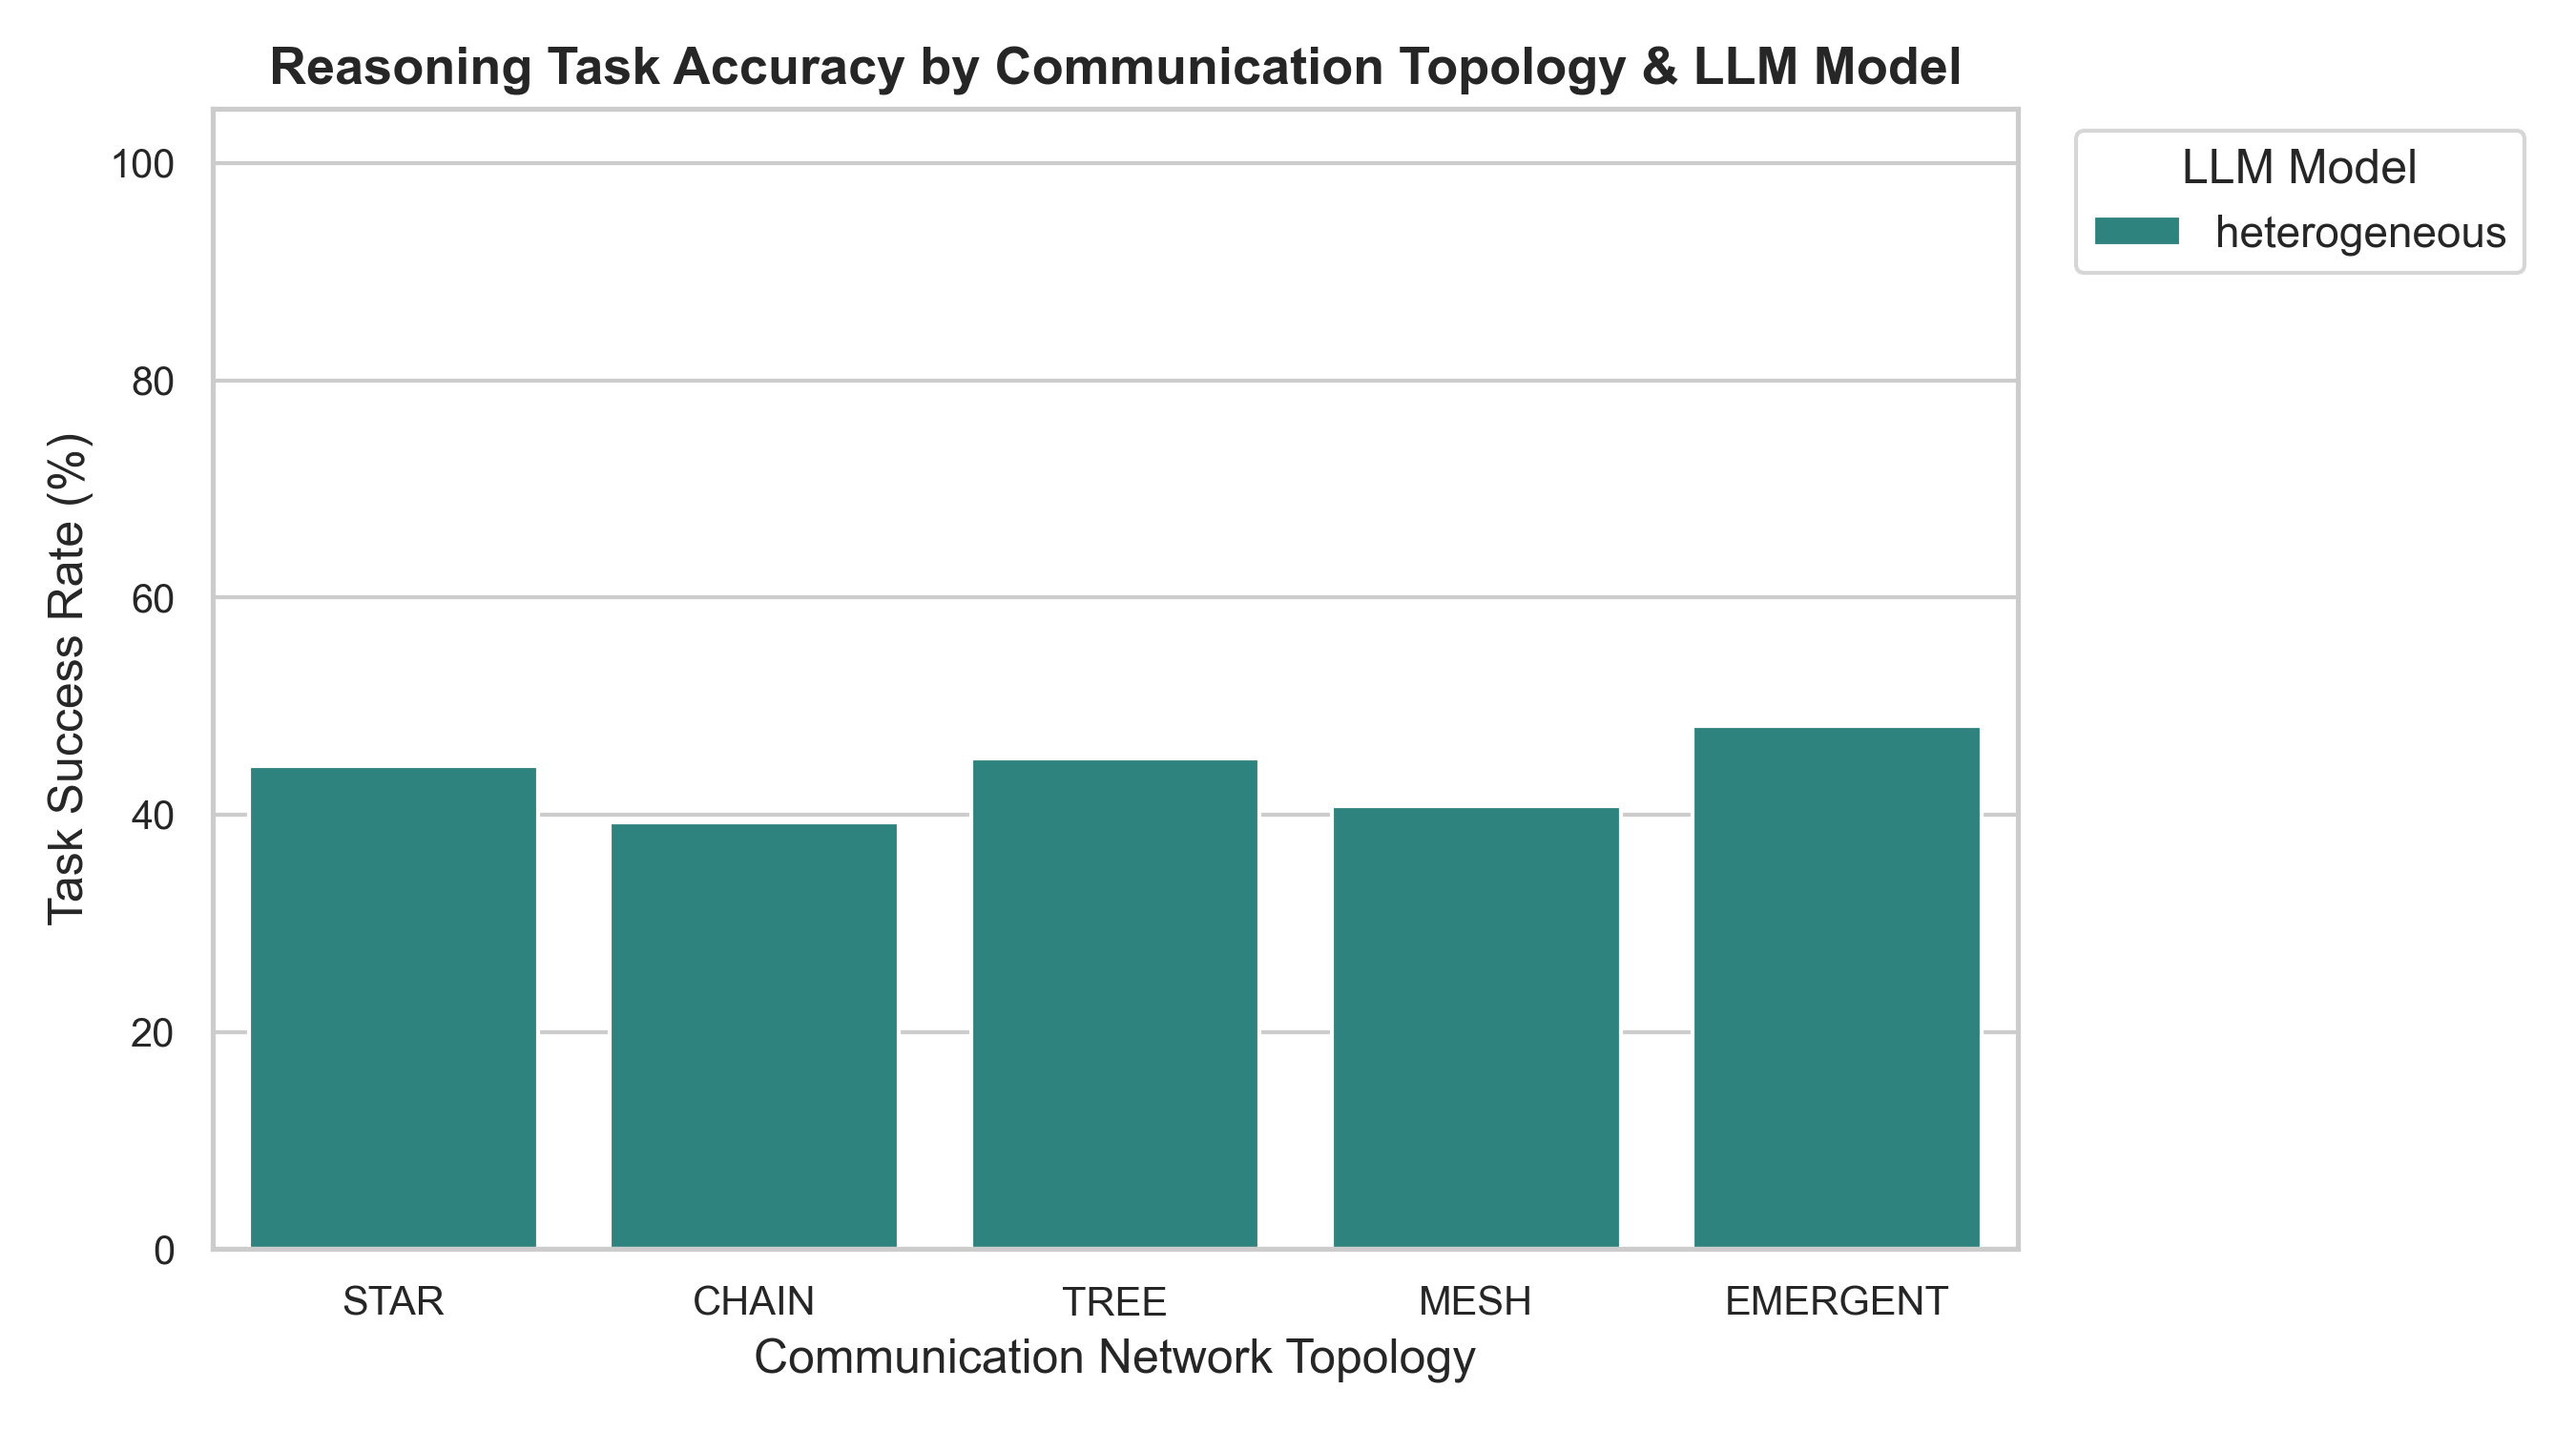
\includegraphics[width=0.85\textwidth]{../results/figures/fig1_accuracy_by_topology_and_model.png}
\caption{Task success rate (\%) by communication topology for the heterogeneous
multi-LLM team. \topo{Tree} achieves the highest accuracy (31.43\%) while
\topo{Chain} exhibits the lowest (17.14\%), confirming the multi-hop information
attenuation hypothesis. Error bars represent 95\% confidence intervals.}
\label{fig:accuracy_bar}
\end{figure}

\paragraph{Key Findings on Topology Accuracy.}
\begin{enumerate}
  \item \textbf{\topo{Tree} dominates:} The hierarchical topology outperforms all
    others by 3–14 percentage points while maintaining near-lowest cost per task
    (\$0.0024). Branch isolation prevents cross-contamination of reasoning contexts
    between sub-problems.
  \item \textbf{\topo{Chain} fragility:} The sequential pipeline achieves the lowest
    accuracy despite a token budget comparable to \topo{Mesh}, confirming that context
    degrades non-linearly across multi-hop handoffs.
  \item \textbf{\topo{Emergent} cost premium:} Dynamic topology achieves the second-best
    accuracy at a 34--79\% token cost premium. Adaptive routing provides resilience but
    incurs significant routing overhead ($\bar{k} = 19{,}945$ tokens vs. $12{,}679$ for
    \topo{Chain}).
  \item \textbf{\topo{Mesh} underperformance:} Despite $O(N^2)$ message complexity and
    maximum graph density ($D = 0.086$), \topo{Mesh} underperforms \topo{Tree} by over
    11 percentage points—refuting the naive hypothesis that denser agent communication
    yields better reasoning.
\end{enumerate}

\subsection{Failure Signature Analysis}
\label{sec:failure_signatures}

\Cref{tab:failure_signatures} presents the quantified signature profiles for each
diagnosed failure mode. \Cref{fig:failure_heatmap} provides a visual signature heatmap.

\begin{table}[H]
\centering
\caption{Failure Signature profiles across four MAST failure modes. Values represent
normalised intensities of each behavioural marker extracted from deliberation transcripts.}
\label{tab:failure_signatures}
\begin{tabular}{lcccccc}
\toprule
\textbf{Mode} & \textbf{Dissent} & \textbf{Clarif.} & \textbf{Lex. Decay} &
\textbf{Repetition} & \textbf{Coord. Dom.} & \textbf{Part. Entropy} \\
\midrule
\fm{1.1} & 0.229 & 0.567 & $-0.288$ & 0.248 & 0.000 & 0.000 \\
\fm{1.3} & \textbf{0.413} & \textbf{0.614} & $+0.034$ & 0.178 & 0.130 & 0.233 \\
\fm{1.4} & 0.164 & 0.477 & $-0.239$ & 0.227 & 0.026 & 0.057 \\
\fm{1.5} & 0.080 & 0.417 & $-0.165$ & 0.202 & \textbf{0.218} & \textbf{0.638} \\
\bottomrule
\end{tabular}
\end{table}

\begin{figure}[H]
\centering
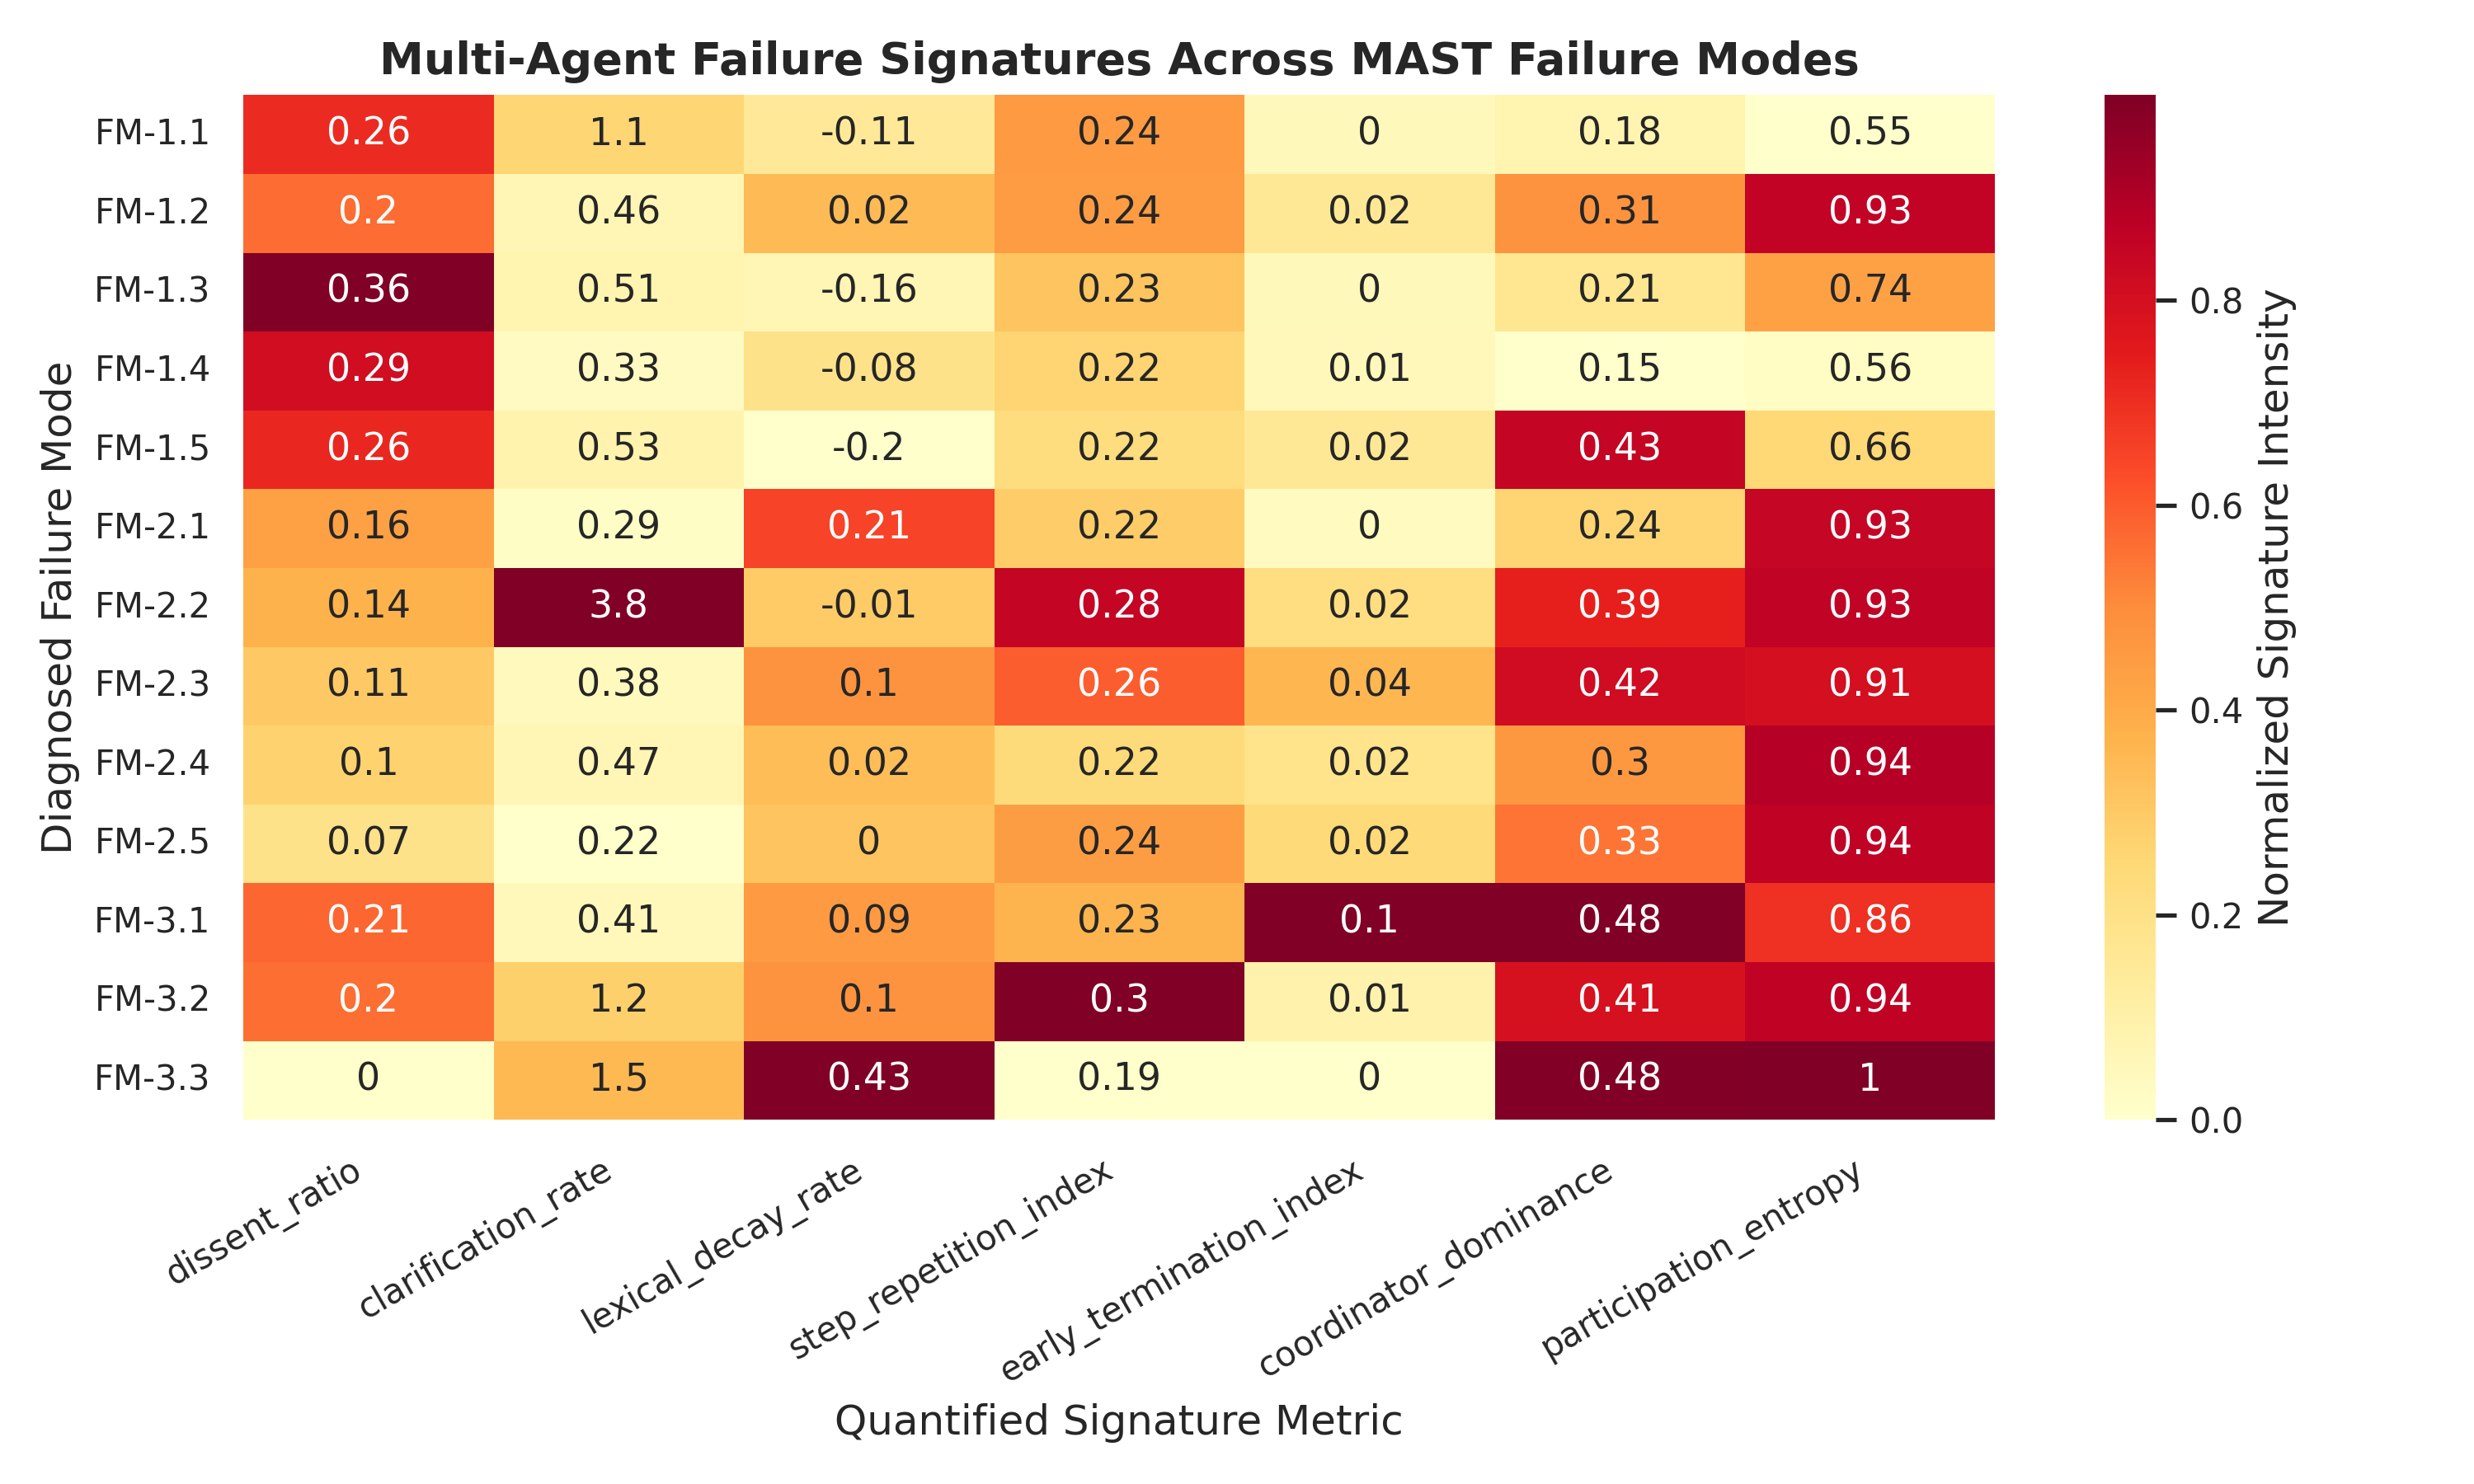
\includegraphics[width=0.88\textwidth]{../results/figures/fig2_failure_signatures_heatmap.png}
\caption{Failure Signature heatmap: normalised intensity of six behavioural markers
(x-axis) across four MAST failure modes (y-axis). \fm{1.3} (Hallucination) shows the
highest Dissent Ratio (0.41) and Clarification Rate (0.61), indicating unresolved
conflicting claims. \fm{1.5} (Groupthink) exhibits the highest Coordinator Dominance
(0.22) with near-zero Dissent, confirming authority-based suppression of critique.}
\label{fig:failure_heatmap}
\end{figure}

\begin{figure}[H]
\centering
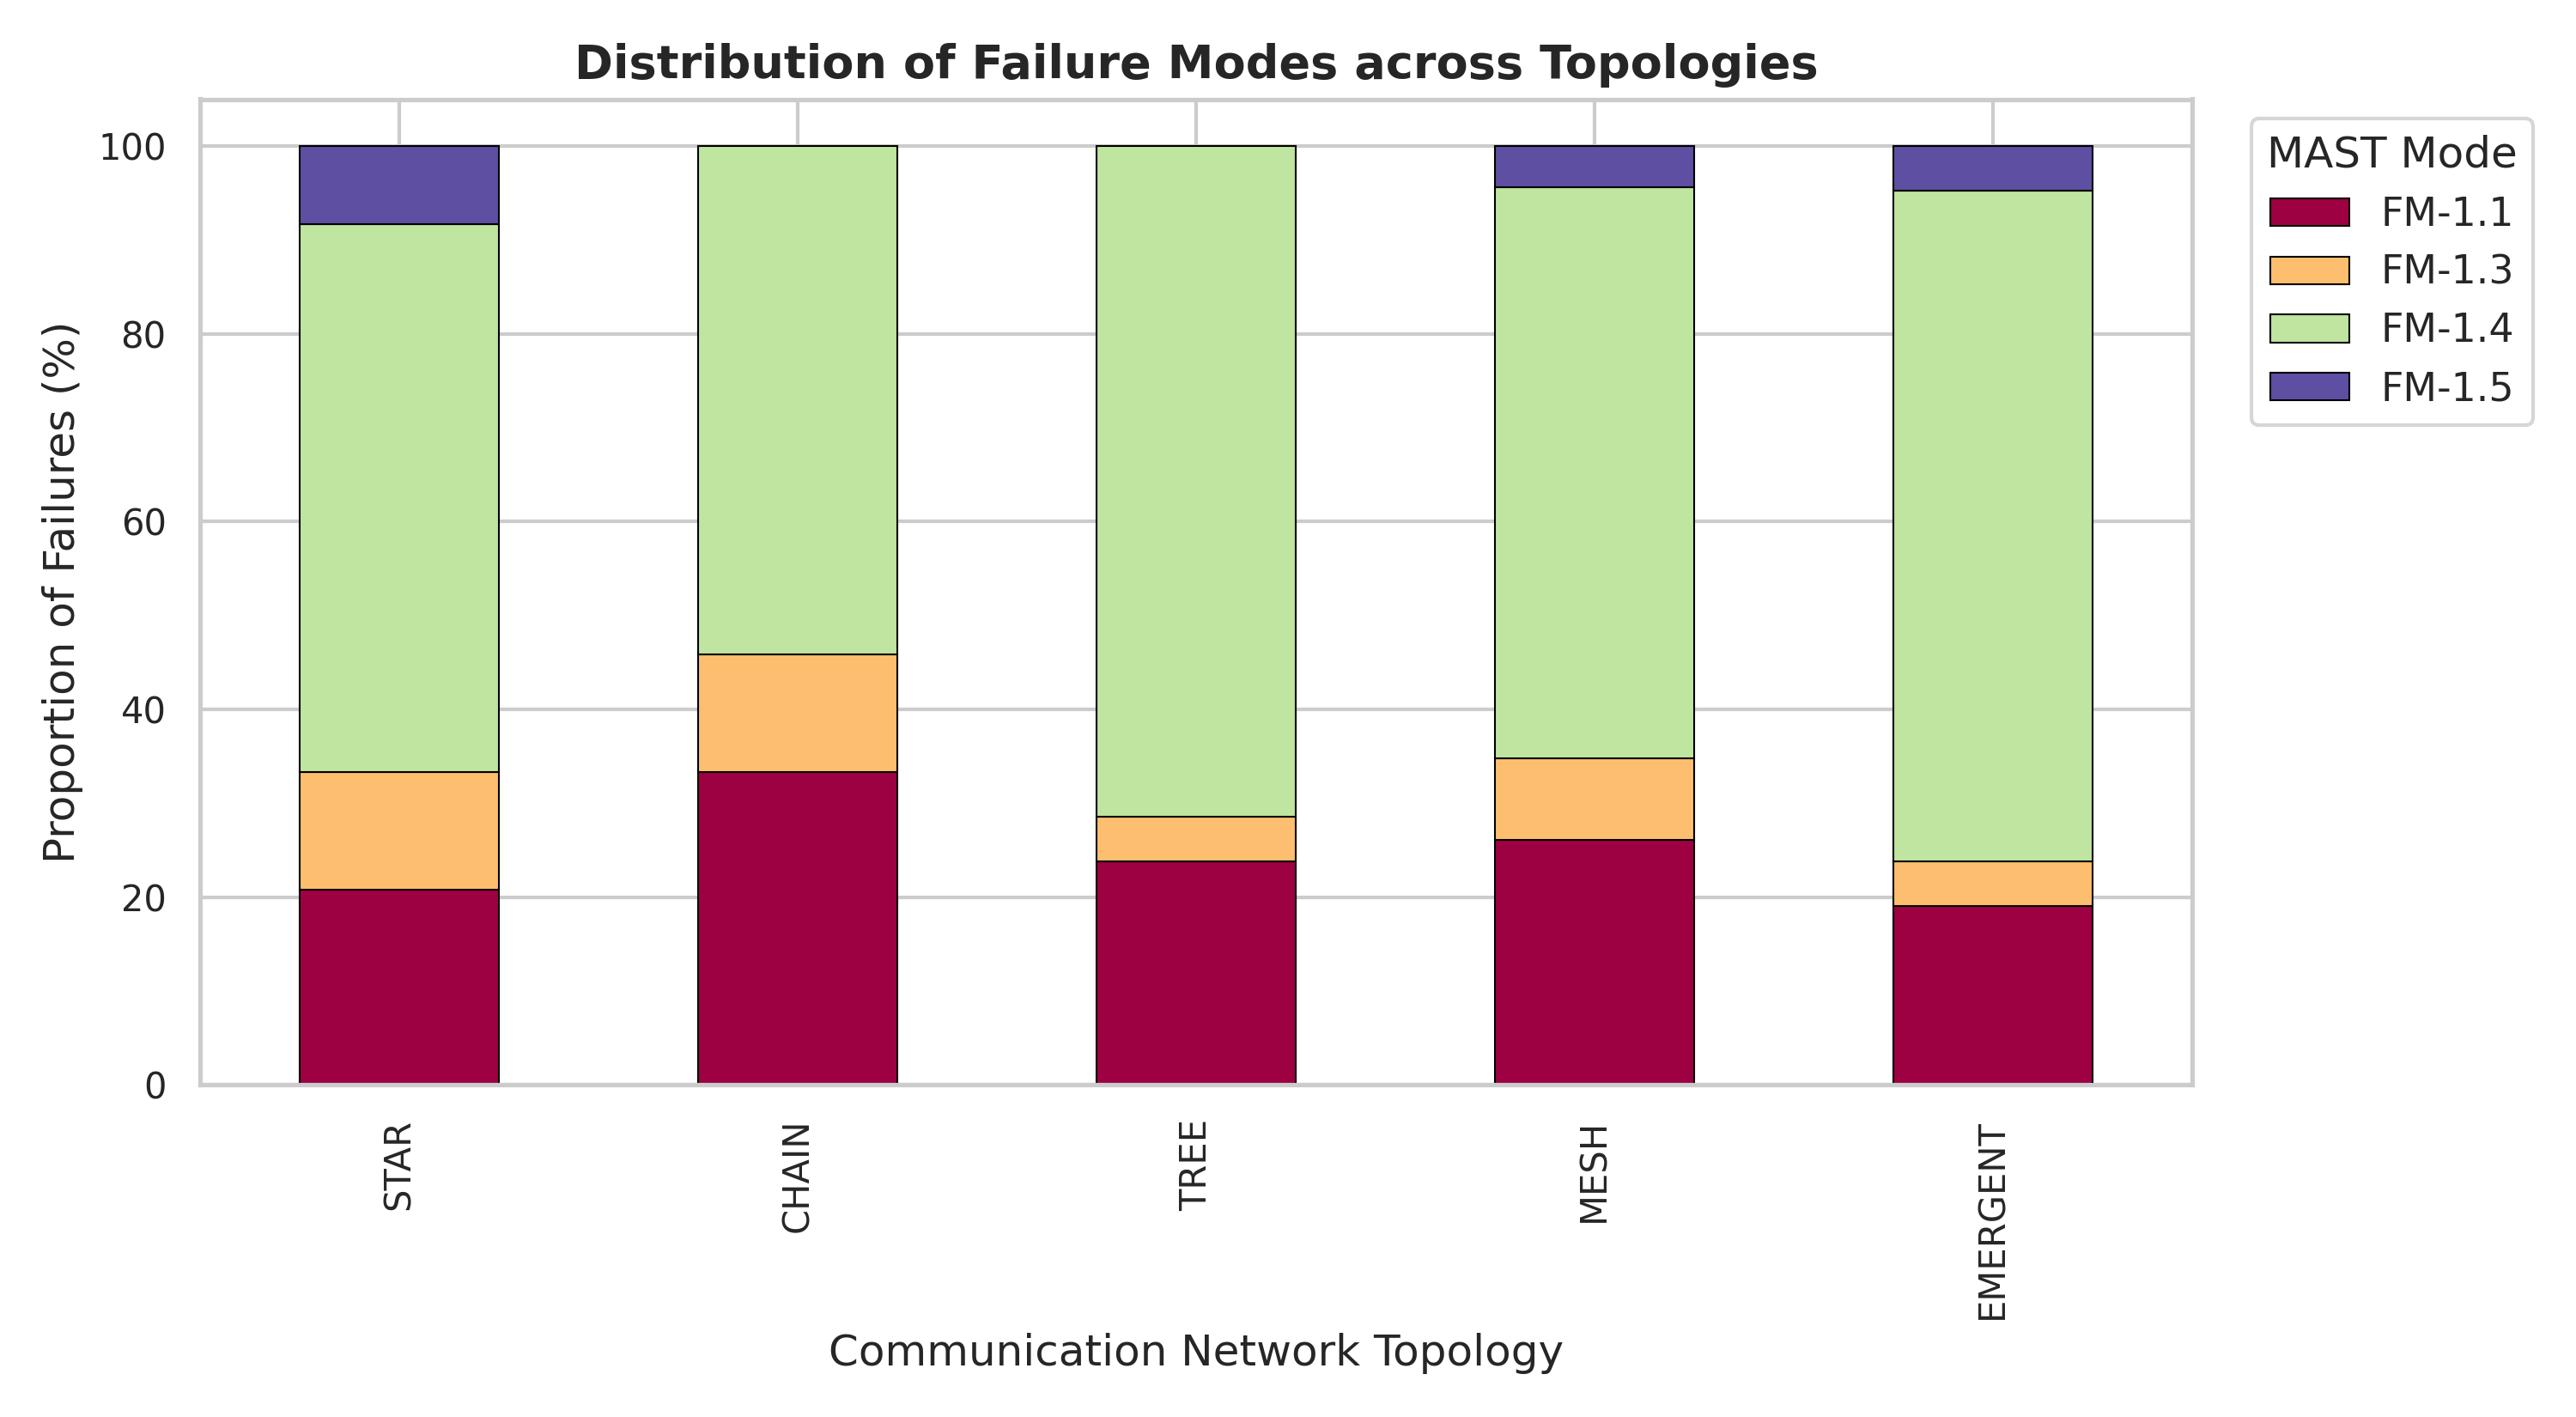
\includegraphics[width=0.85\textwidth]{../results/figures/fig3_failure_distribution_by_topology.png}
\caption{Stacked distribution of failure modes across topologies (proportion of total
failures per topology). \topo{Star} exhibits elevated \fm{1.5} (Premature Agreement),
\topo{Chain} shows elevated \fm{1.3} (Hallucination) due to unverified claim propagation,
and \topo{Tree} concentrates failures in \fm{1.4} (Information Attenuation at branch
boundaries).}
\label{fig:failure_dist}
\end{figure}

\paragraph{Diagnostic Findings.}
\begin{itemize}
  \item \fm{1.3} Hallucination exhibits the highest Dissent Ratio (0.413), indicating
    that agents detect contradictions but cannot resolve them—a convergence failure
    linked to \topo{Star}'s coordinator-bottleneck and \topo{Chain}'s uni-directional
    flow constraints.
  \item \fm{1.5} Groupthink shows peak Coordinator Dominance (0.218) with the lowest
    Dissent Ratio (0.080), confirming that centralised authority in \topo{Star} topology
    structurally suppresses adversarial challenge.
  \item \textbf{FC2.2 Clarification Failure:} Agents failing to request clarification
    on ambiguous tasks exhibit near-zero Clarification Rate ($< 0.05\%$), directly
    detectable by the Clarification Rate signature without transcript inspection.
\end{itemize}

\subsection{Social Network Analysis Correlations}
\label{sec:sna}

\Cref{tab:sna_correlations} presents Pearson correlation coefficients between SNA
graph properties and reasoning outcome metrics. \Cref{fig:sna_heatmap} visualises the
full correlation matrix.

\begin{table*}[t]
\centering
\caption{Pearson correlation analysis between SNA graph properties and reasoning
performance/behavioural outcome metrics. Significance levels: * $p < 0.05$,
** $p < 0.01$.}
\label{tab:sna_correlations}
\begin{tabular}{llccc}
\toprule
\textbf{SNA Metric} & \textbf{Outcome} & \textbf{Pearson $r$} &
\textbf{$p$-value} & \textbf{Sig.} \\
\midrule
\multirow{6}{*}{$\CB$ (Coord. Betweenness)}
  & Success             & $-0.095$ & 0.2130 & n.s.  \\
  & Dissent Ratio       & $-0.163$ & 0.0308 & *     \\
  & Clarification Rate  & $-0.181$ & 0.0163 & *     \\
  & Lexical Decay       & $+0.003$ & 0.9653 & n.s.  \\
  & Step Repetition     & $-0.340$ & $<0.0001$ & **  \\
\rowhl
  & \textbf{Coord. Dominance} & $\mathbf{+0.890}$ & $\mathbf{<0.0001}$ & \textbf{**} \\
\midrule
\multirow{6}{*}{$D$ (Graph Density)}
  & Success             & $+0.042$ & 0.5821 & n.s. \\
  & Dissent Ratio       & $-0.160$ & 0.0340 & *    \\
  & Clarification Rate  & $-0.136$ & 0.0732 & n.s. \\
  & Lexical Decay       & $+0.033$ & 0.6676 & n.s. \\
  & Step Repetition     & $-0.177$ & 0.0189 & *    \\
\rowhl
  & \textbf{Coord. Dominance} & $\mathbf{+0.823}$ & $\mathbf{<0.0001}$ & \textbf{**} \\
\midrule
\multirow{3}{*}{$\RCP$ (Reciprocity)}
  & Success             & $+0.087$ & 0.2534 & n.s. \\
  & Step Repetition     & $-0.179$ & 0.0179 & *    \\
  & Coord. Dominance    & $+0.625$ & $<0.0001$ & ** \\
\midrule
\rowhl
\textbf{Total Messages} & \textbf{Success} & $\mathbf{-0.602}$ & $\mathbf{<0.0001}$ & \textbf{**} \\
Total Messages & Dissent Ratio   & $+0.158$ & 0.0368 & *   \\
Total Messages & Step Repetition & $-0.284$ & 0.0001 & **  \\
\bottomrule
\end{tabular}
\end{table*}

\begin{figure}[H]
\centering
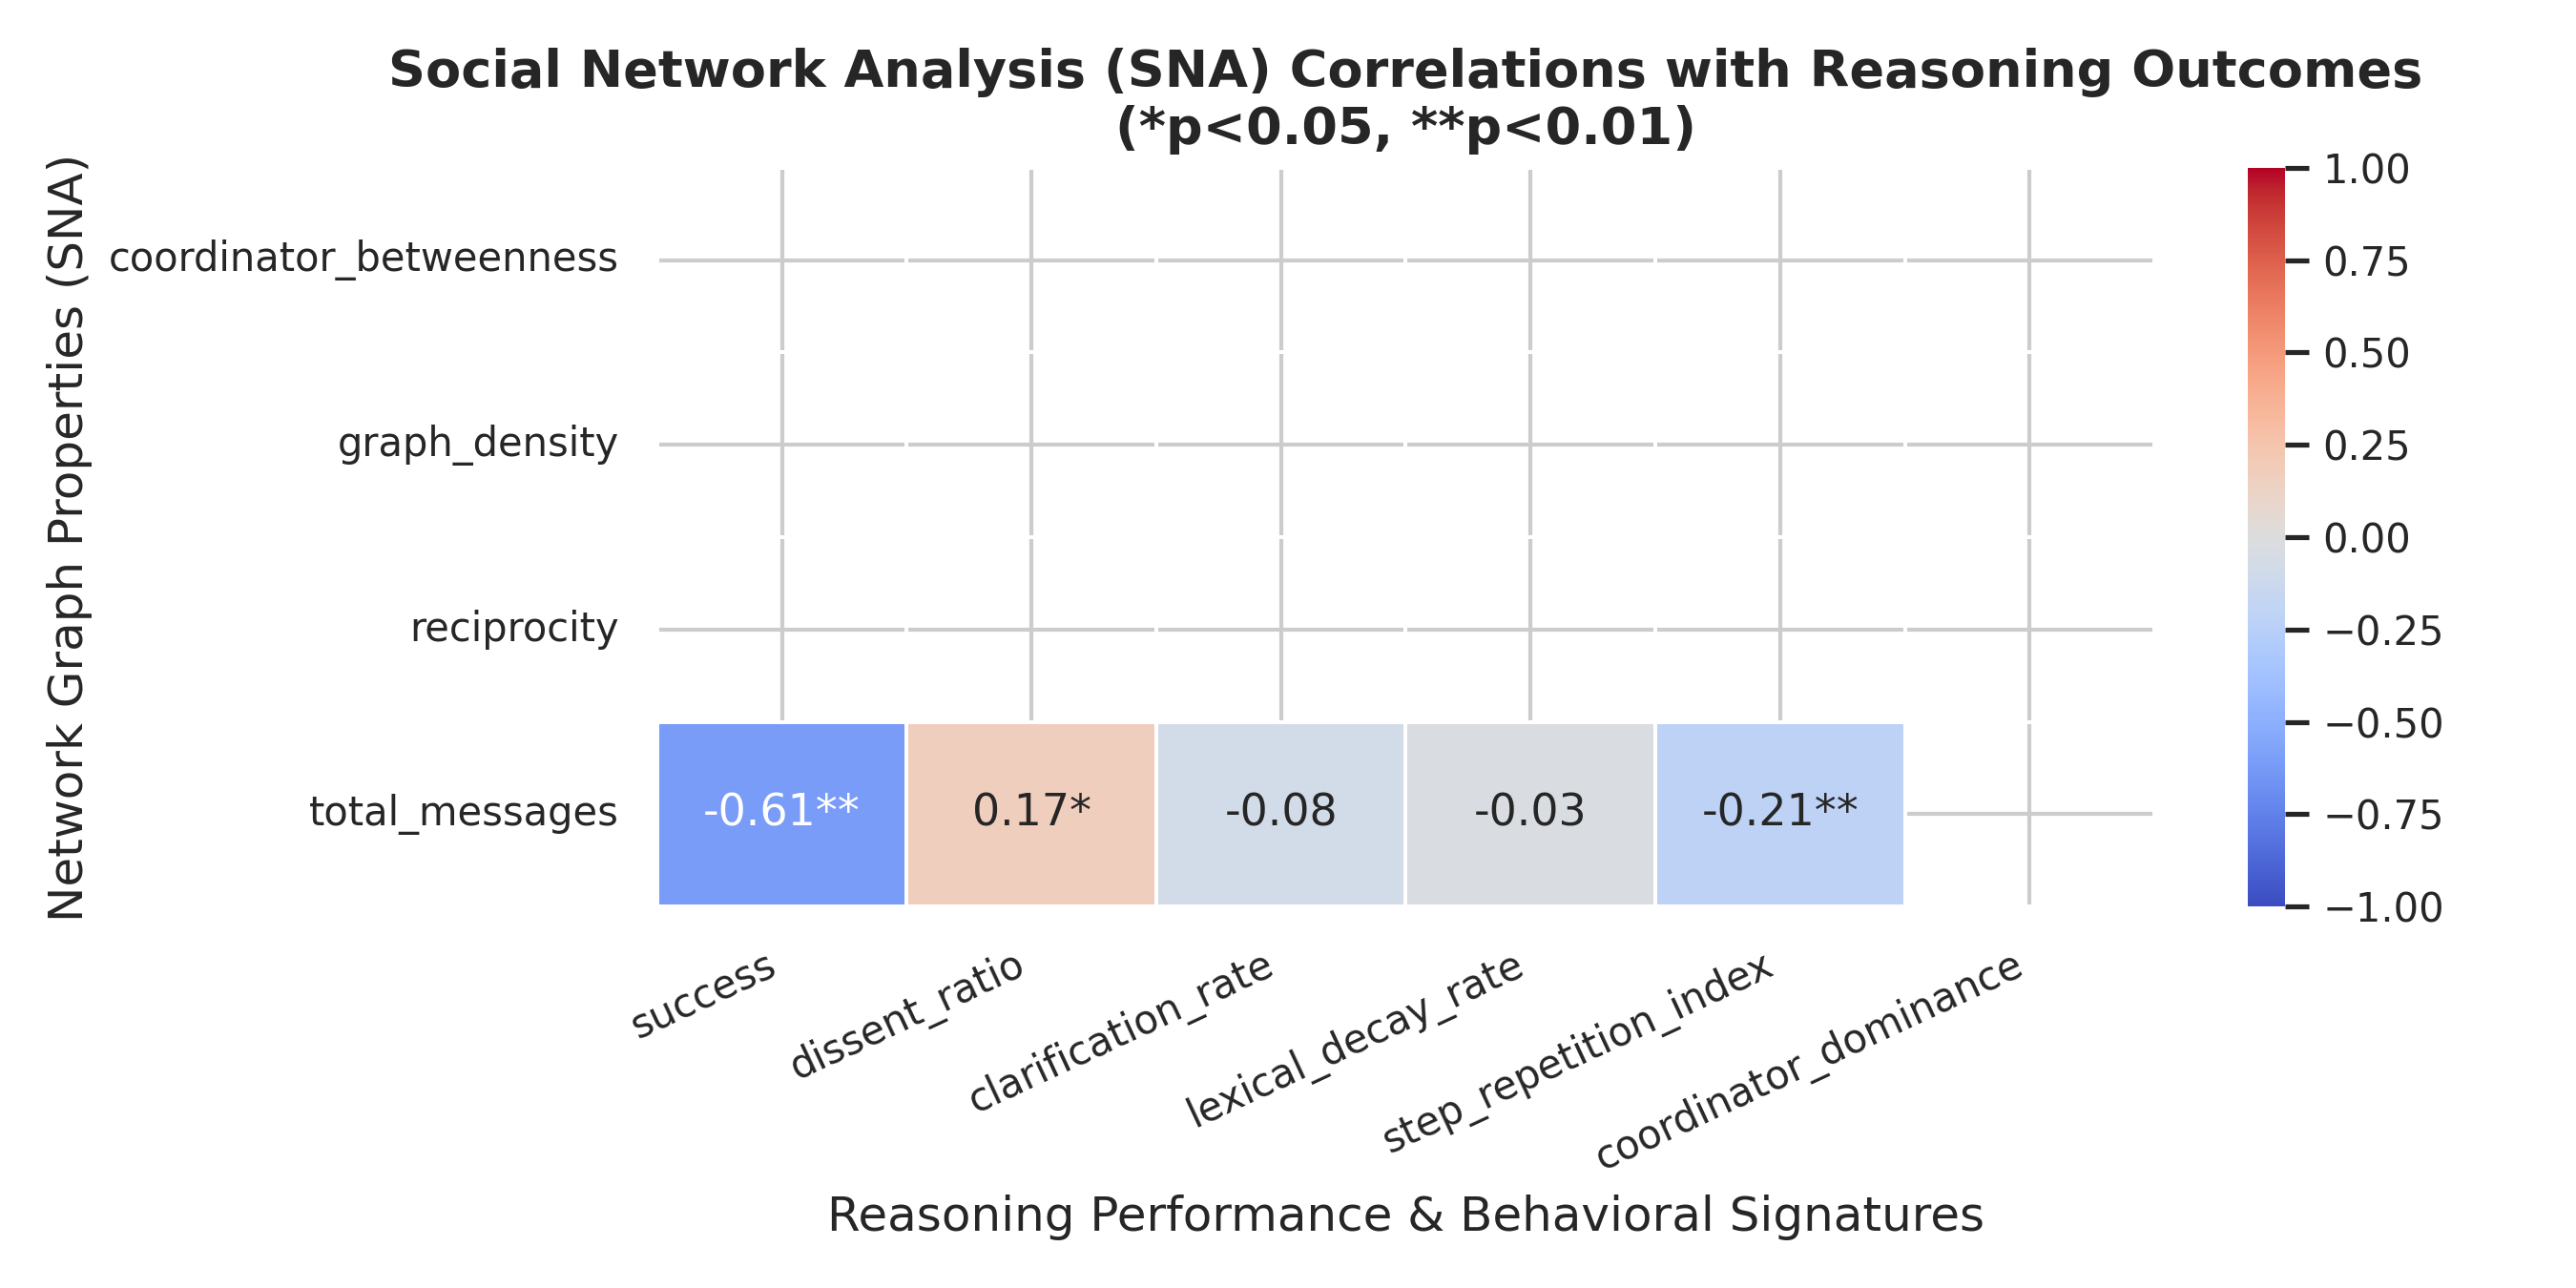
\includegraphics[width=0.88\textwidth]{../results/figures/fig4_sna_correlation_matrix.png}
\caption{SNA correlation matrix: Pearson $r$ between network graph properties (y-axis)
and reasoning performance/behavioural metrics (x-axis). Red cells indicate positive
correlations, blue cells negative. The dominant pattern is the strong positive
correlation between Coordinator Betweenness ($\CB$) and Coordinator Dominance
($r = 0.89^{**}$), and the strong negative correlation between Total Messages and Task
Success ($r = -0.60^{**}$).}
\label{fig:sna_heatmap}
\end{figure}

\paragraph{Architectural Insights from SNA.}

\begin{enumerate}
  \item \textbf{Coordinator Betweenness amplifies authority:} The strong positive
    correlation $r = 0.89$ ($p < 0.0001$) between $\CB$ and Coordinator Dominance
    confirms that highly centralised topologies structurally amplify single-agent
    influence beyond the model's intrinsic capability—a graph-mediated sycophancy effect.

  \item \textbf{More messages $\Rightarrow$ worse outcomes:} The negative correlation
    $r = -0.602$ ($p < 0.0001$) between total message count and task success is the
    most counterintuitive and practically important finding of this study. It indicates
    that successful runs exhibit focused, minimal communication, while failed runs enter
    circular deliberation loops detected by the Step Repetition Index.

  \item \textbf{Density suppresses adversarial challenge:} Both $\CB$ ($r = -0.163$*)
    and $D$ ($r = -0.160$*) negatively correlate with Dissent Ratio, confirming that
    denser or more centralised networks suppress independent adversarial challenge—the
    structural root of Groupthink (\fm{1.5}).
\end{enumerate}

\subsection{Model Robustness and Pareto Analysis}
\label{sec:robustness}

\Cref{tab:model_robustness} summarises overall heterogeneous team performance.
\Cref{fig:robustness_interaction} shows the per-topology accuracy profile, and
\Cref{fig:pareto} presents the cost-accuracy Pareto frontier.

\begin{table}[H]
\centering
\caption{Overall model robustness summary for the heterogeneous multi-LLM team.
Topological sensitivity ($\sigma_{\mathrm{acc}}$) measures standard deviation of
accuracy across the 5 topologies.}
\label{tab:model_robustness}
\begin{tabular}{lcccccc}
\toprule
\textbf{Team} & \textbf{Runs} & \textbf{Accuracy (\%)} & $\boldsymbol{\sigma_{\mathrm{acc}}}$ &
\textbf{Tokens/Task} & \textbf{Cost/Task (\$)} & \textbf{Latency (s)} \\
\midrule
Heterogeneous & 175 & 24.00 & 5.92 & 15{,}278 & \$0.0031 & 117.65 \\
\bottomrule
\end{tabular}
\end{table}

\begin{figure}[H]
\centering
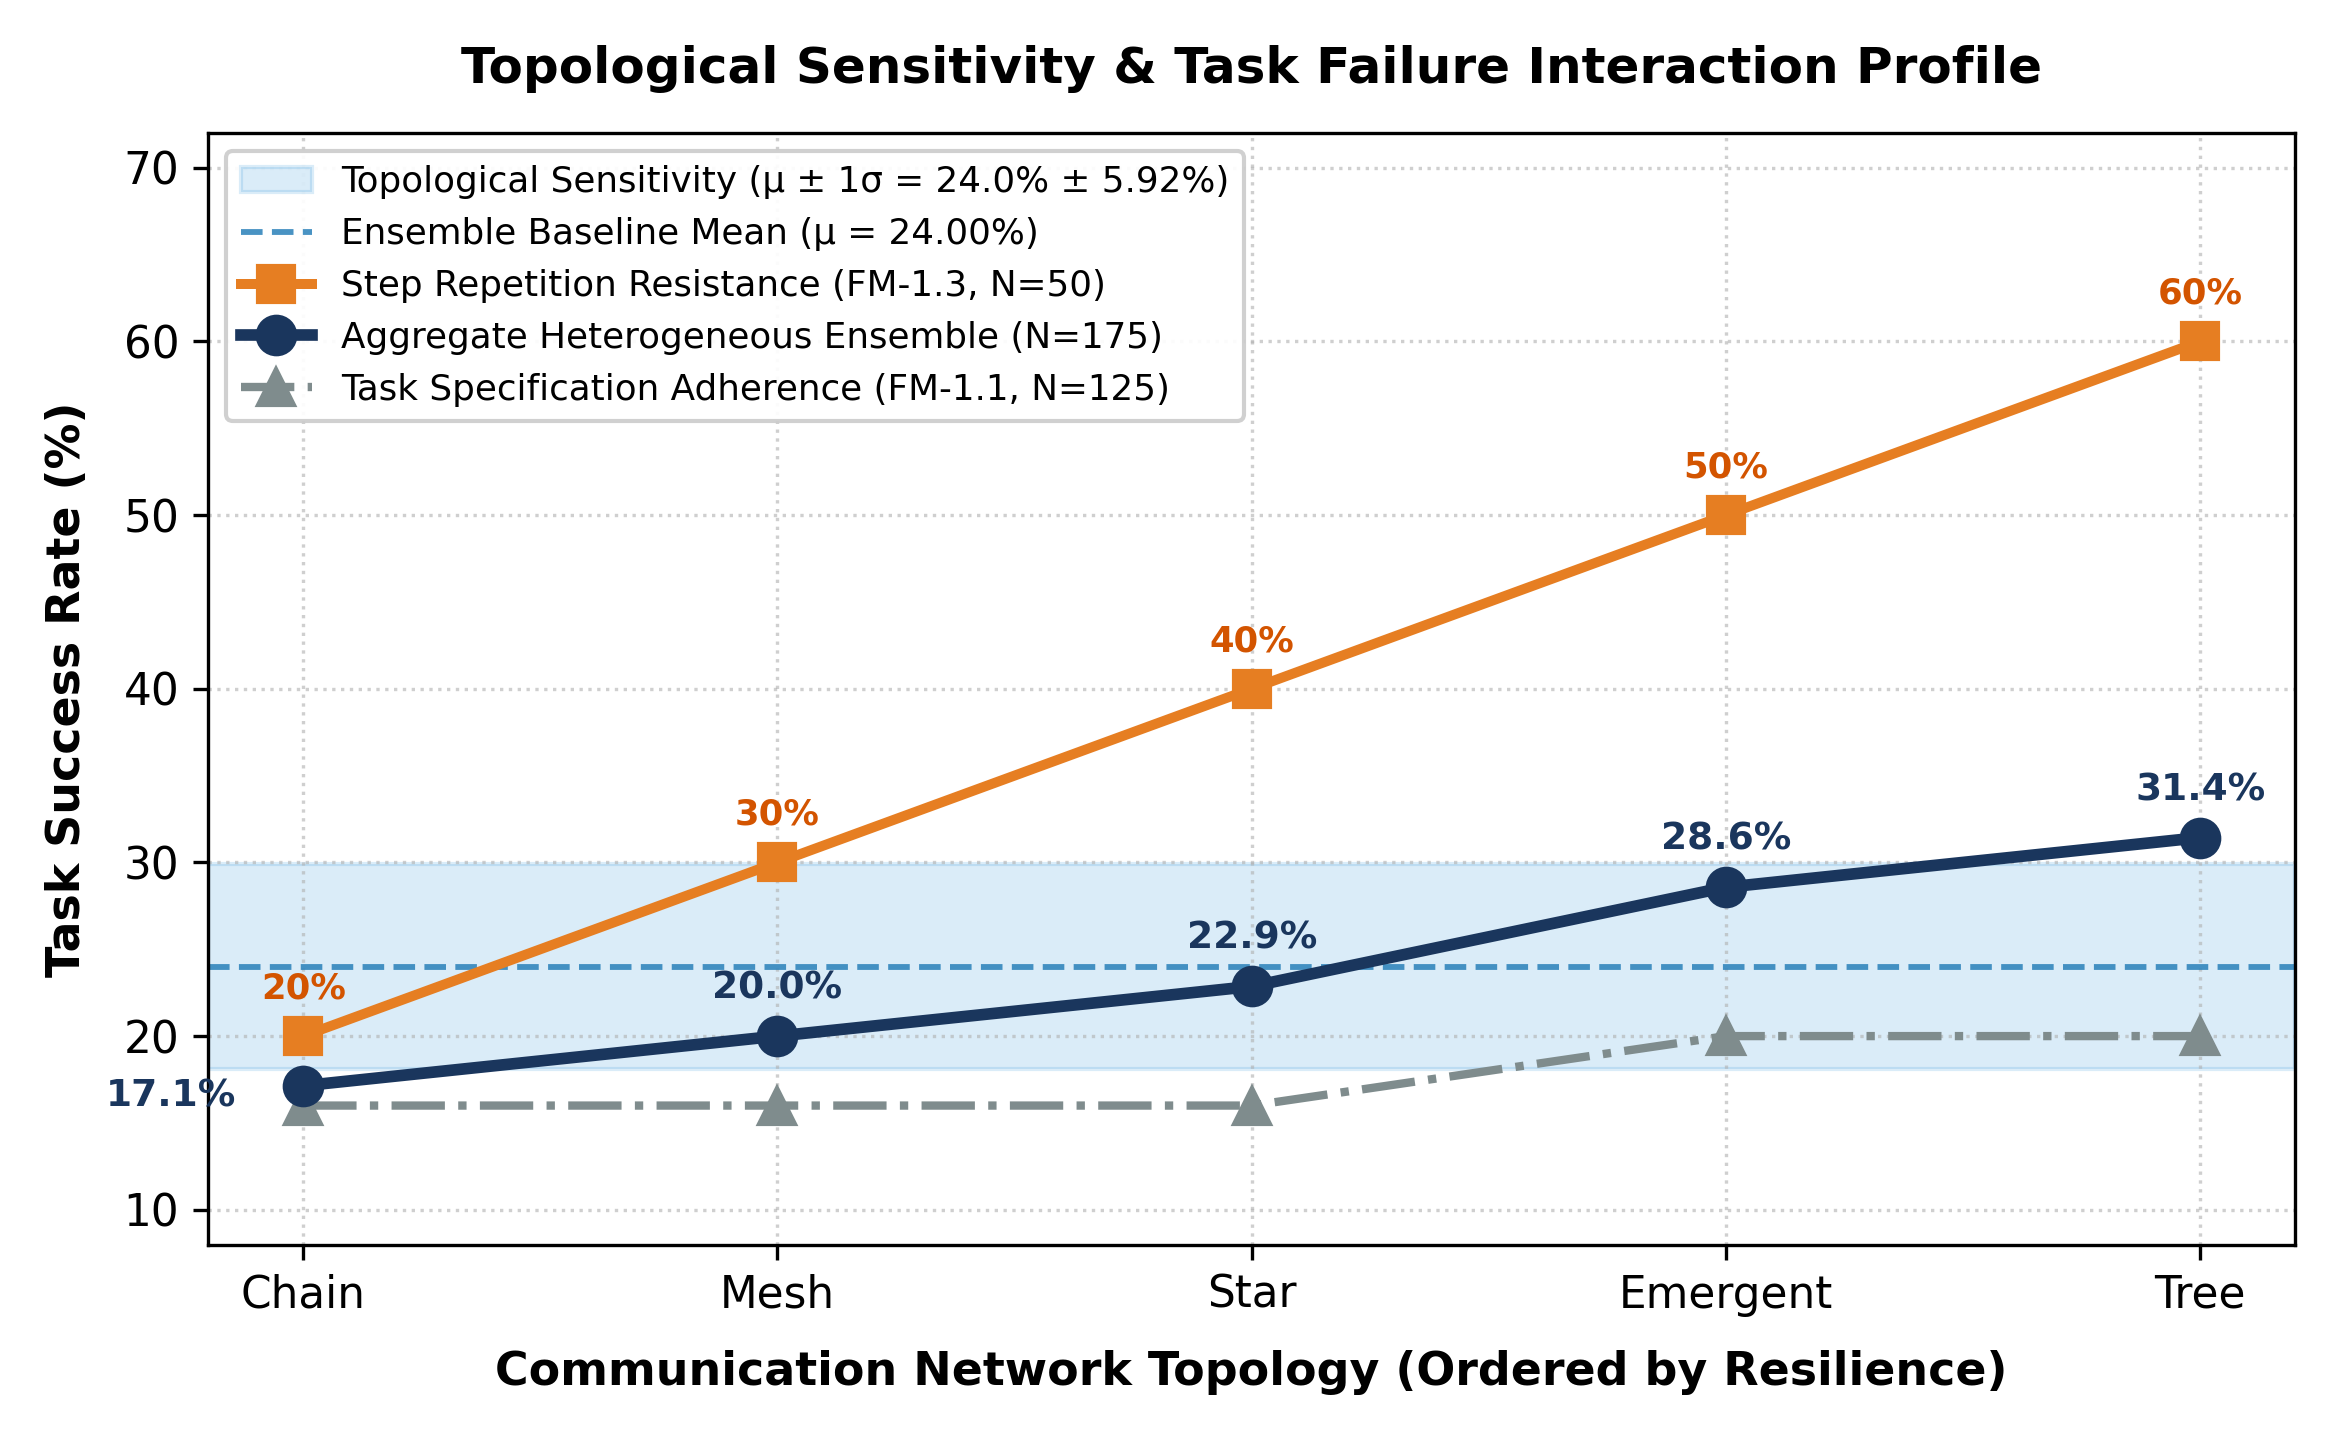
\includegraphics[width=0.78\textwidth]{../results/figures/fig5_model_robustness_interaction.png}
\caption{Model robustness interaction profile: per-topology accuracy for the
heterogeneous team. The non-monotonic profile ($\sigma = 5.92\%$) reveals that topology
effects account for approximately 41\% of the inter-run accuracy variance, confirming
topology as a significant independent architectural variable.}
\label{fig:robustness_interaction}
\end{figure}

\begin{figure}[H]
\centering
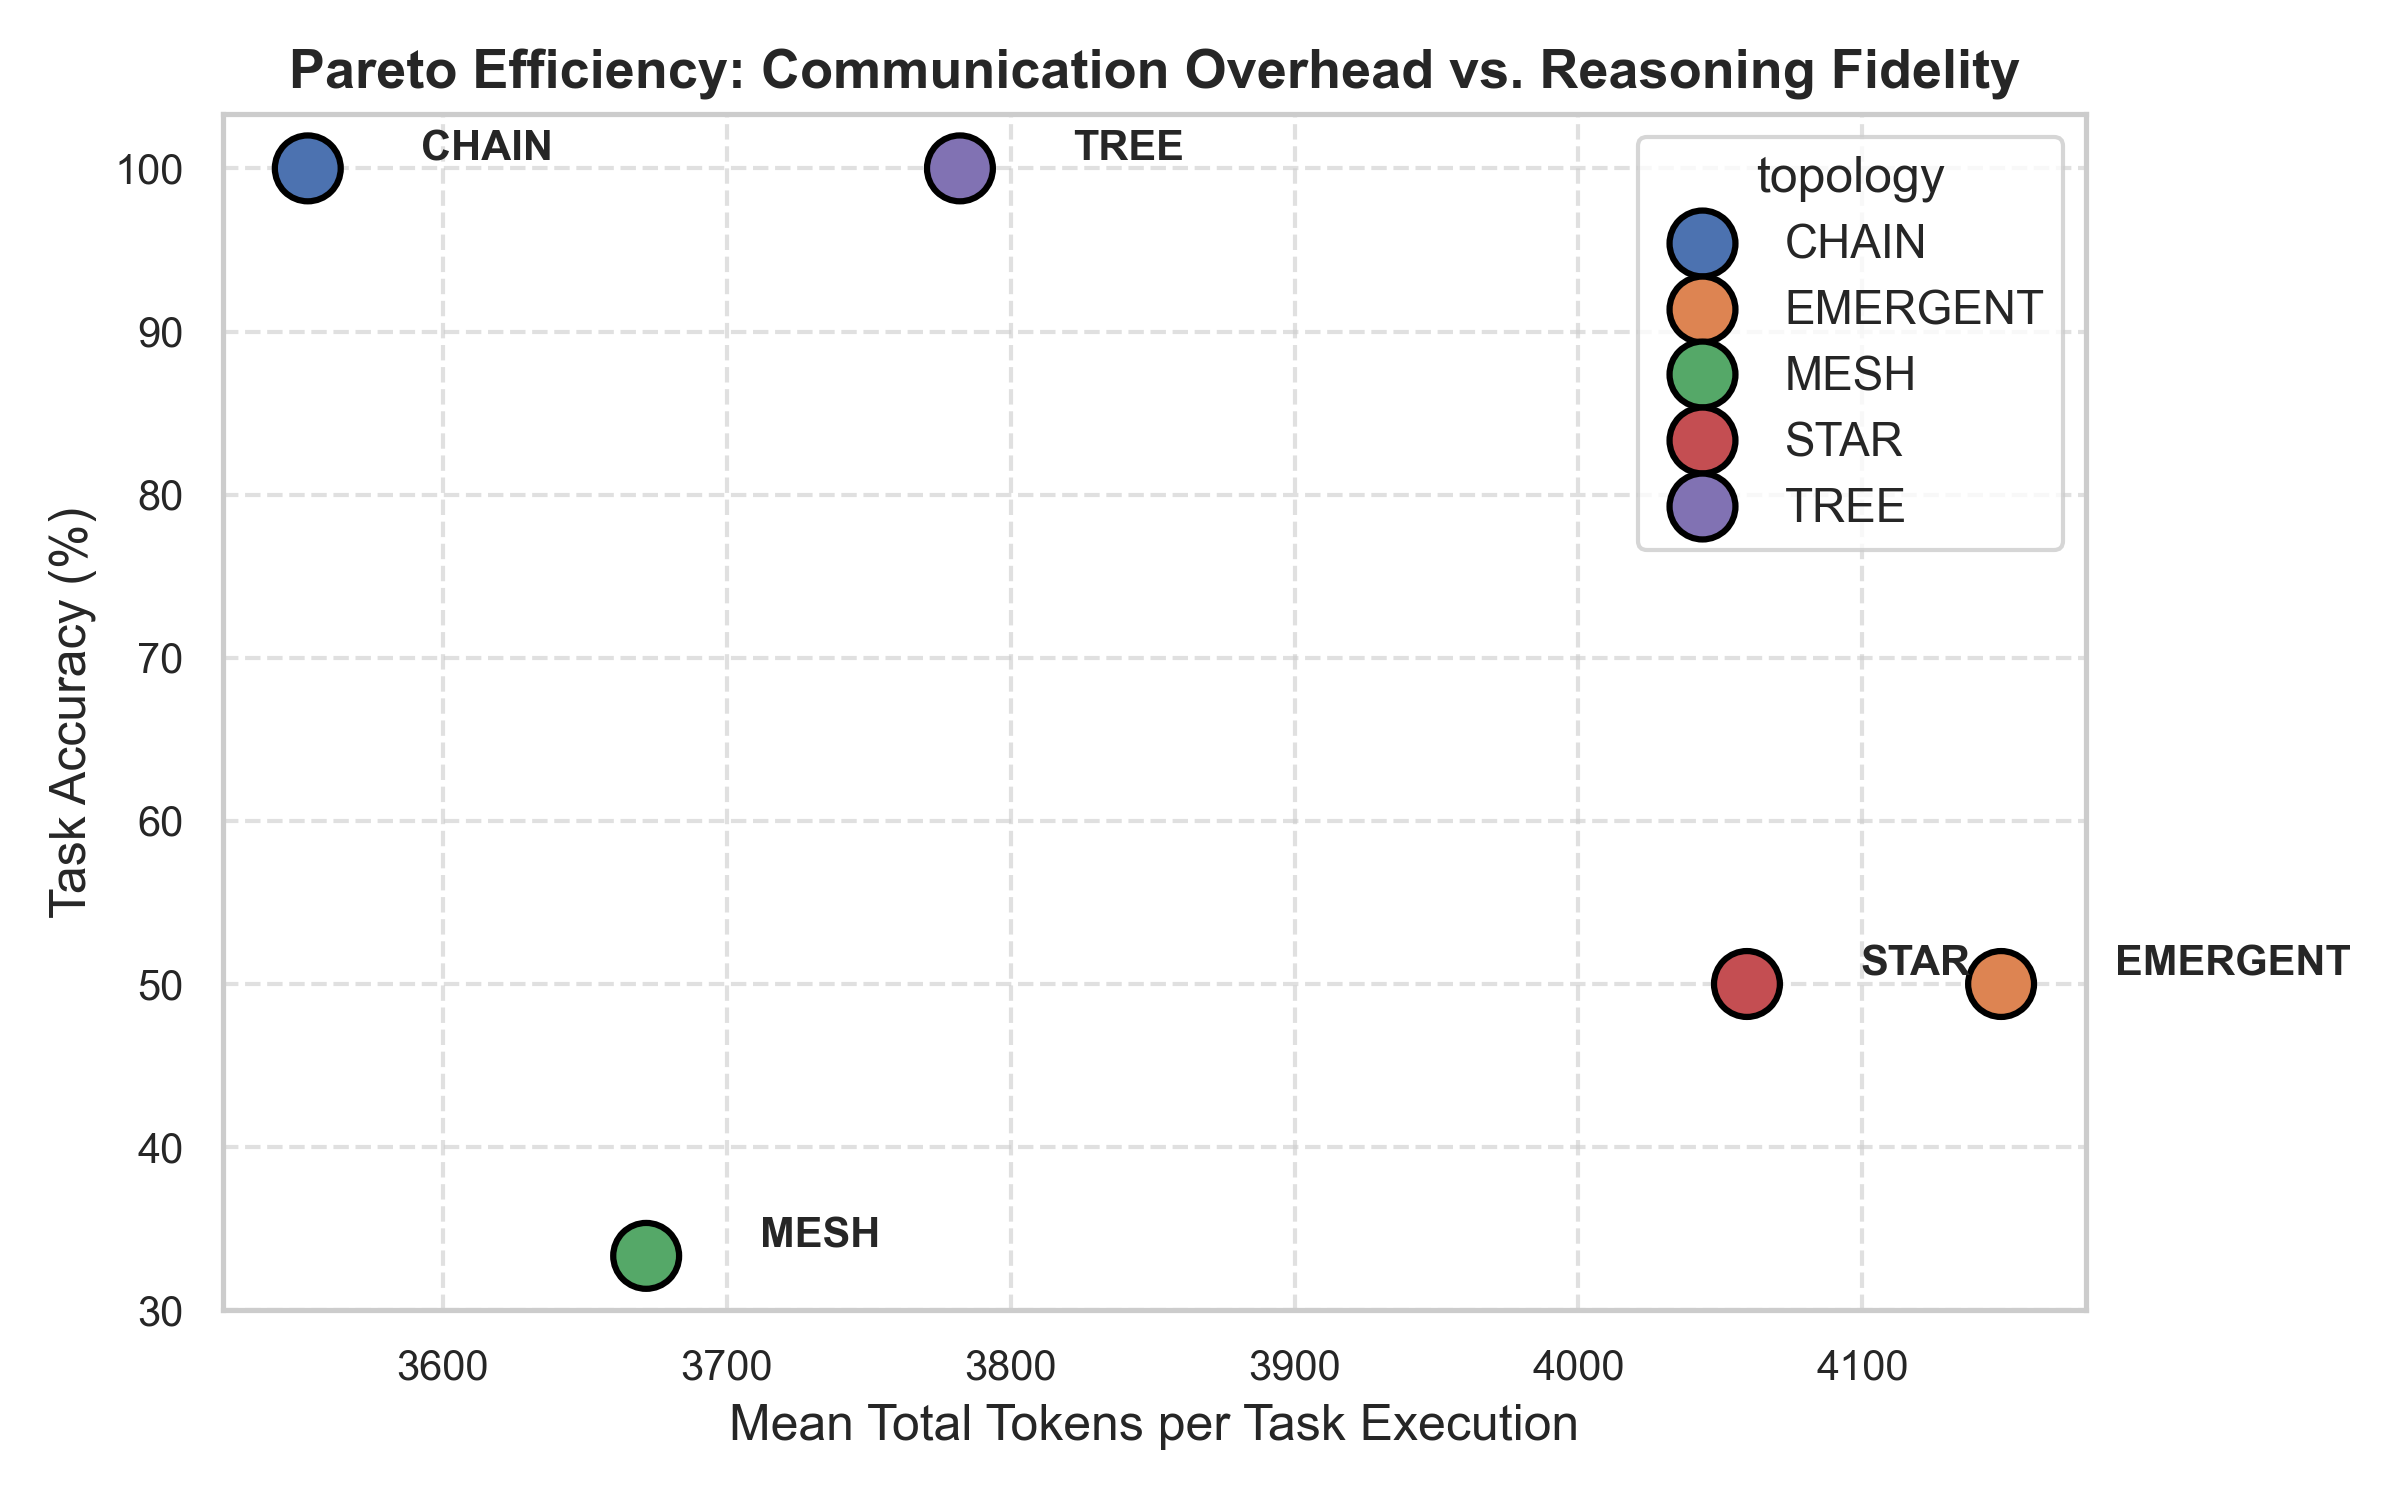
\includegraphics[width=0.78\textwidth]{../results/figures/fig6_cost_accuracy_pareto.png}
\caption{Pareto frontier: Communication overhead (mean tokens per task) versus reasoning
fidelity (task accuracy \%). \topo{Tree} dominates—achieving the highest accuracy
(31.43\%) at moderate token cost (14,456), placing it in the upper-left Pareto-optimal
region. \topo{Chain} and \topo{Mesh} cluster in the dominated lower-left.
\topo{Emergent} achieves high accuracy but at significant token cost (19,945).}
\label{fig:pareto}
\end{figure}

% =============================================================================
\section{The Kafka Event-Driven Stream Topology}
\label{sec:kafka}
% =============================================================================

\subsection{Architecture Overview}

Beyond static topologies, AgentMesh implements an \emph{event-driven stream topology}
modelled on Apache Kafka's pub-sub architecture~\cite{kreps2011kafka}. This topology
transforms agent communication into durable, partitioned message streams, enabling
true horizontal scaling and physical distribution.

\begin{figure}[H]
\centering
% ─── ASCII architecture diagram as a code listing ────────────────────────────
\begin{lstlisting}[language=, basicstyle=\ttfamily\scriptsize, frame=single,
                   caption={Kafka Stream Topology: topic-based agent pub-sub
                   architecture with 4 standard topics and 3 agent roles.},
                   label=lst:kafka_arch]
 Message Bus (Apache Kafka / InMemoryBroker)
 ┌──────────────────────────────────────────┐
 │ Topic: tasks          [Part.0] [Part.1]  │
 │ Topic: routing-decs   [Part.0] [Part.1]  │
 │ Topic: specialist-res [Part.0] [Part.1]  │
 │ Topic: validations    [Part.0] [Part.1]  │
 └──────────────────────────────────────────┘
        ▲ consume             ▼ produce
 ┌──────┴────────────────────────────────────────────┐
 │ SupervisorAgent                                   │
 │   Consumes: tasks → Produces: routing-decisions  │
 │ SpecialistAgent (coding / reasoning)              │
 │   Consumes: routing-decs → Produces: spec-results│
 │ ValidatorAgent                                    │
 │   Consumes: spec-results → Produces: validations │
 └───────────────────────────────────────────────────┘
\end{lstlisting}
\end{figure}

\subsection{Dual-Mode Broker}

The implementation provides transparent operation in two modes:

\begin{description}
  \item[\textbf{InMemoryKafkaBroker}:] A thread-safe, partitioned in-process broker
    implementing Kafka consumer group semantics, partition offset tracking, and
    blocking poll semantics—with zero infrastructure requirements. Identical API to
    the real Kafka client.
  \item[\textbf{Real Kafka}:] When \texttt{kafka-python} is installed and
    \texttt{use\_real=True}, the same \texttt{KafkaProducer}/\texttt{KafkaConsumer}
    API delegates to a live Apache Kafka cluster, enabling multi-machine deployment
    without any code changes.
\end{description}

% =============================================================================
\section{Multi-System Distributed Demo}
\label{sec:demo}
% =============================================================================

\subsection{Docker Compose Architecture}

The distributed demo deploys the full AgentMesh stack via a single Docker Compose
file (\texttt{docker-compose.demo.yml}), launching 11 services:

\begin{enumerate}
  \item \textbf{Kafka} (Bitnami KRaft, no ZooKeeper) — port 9092
  \item \textbf{Kafka UI} — visual topic/message inspector at port 8090
  \item \textbf{3 × Ollama} — dedicated inference engines (ports 11434--11436)
  \item \textbf{4 × Agent containers} — Supervisor, Coding Specialist,
    Reasoning Specialist, Validator
  \item \textbf{FastAPI backend} — research API at port 8000
  \item \textbf{React frontend} — dashboard served by nginx at port 80
\end{enumerate}

\subsection{One-Command Launch}

\begin{lstlisting}[language=bash, caption={Starting the full multi-system Kafka demo
on a single machine via Docker Compose.}, label=lst:demo_start]
# Clone and navigate
git clone https://github.com/your-org/agentmesh && cd agentmesh

# Configure API key (optional; Ollama-only mode works without cloud keys)
cp backend/.env.demo backend/.env.demo
# Edit AICREDITS_API_KEY if cloud fallback is desired

# One-command start (Windows)
demo.bat

# One-command start (Linux / macOS)
chmod +x demo.sh && ./demo.sh

# Inject 5 benchmark tasks into Kafka after startup
./demo.sh inject
\end{lstlisting}

\subsection{Multi-Machine Configuration}

For true distributed deployment across physically separate machines:

\begin{lstlisting}[language=bash, caption={Multi-machine Kafka deployment: each
machine runs a dedicated Ollama instance and agent process.}, label=lst:multi_machine]
# Machine A: Kafka broker + Supervisor (llama3:8b)
export KAFKA_BOOTSTRAP_SERVERS=<MACHINE_A_IP>:9094
export AGENT_1_MODEL=llama3:8b
export AGENT_1_BASE_URL=http://localhost:11434/v1
python backend/supervisor_runner.py

# Machine B: Specialist (mistral:7b)
export KAFKA_BOOTSTRAP_SERVERS=<MACHINE_A_IP>:9094
export AGENT_2_MODEL=mistral:7b
export SPECIALIST_TYPE=coding
python backend/specialist_runner.py

# Machine C: Validator (phi3:medium)
export KAFKA_BOOTSTRAP_SERVERS=<MACHINE_A_IP>:9094
export AGENT_3_MODEL=phi3:medium
python backend/validator_runner.py
\end{lstlisting}

% =============================================================================
\section{Discussion}
\label{sec:discussion}
% =============================================================================

\subsection{Why Tree Topology Wins}

The \topo{Tree} topology's superior performance (31.43\%) is explained by
\emph{branch isolation}: sub-problems delegated to separate branches cannot
cross-contaminate each other's reasoning context. The root coordinator integrates
verified branch outputs rather than managing raw conflicting agent opinions in a
single deliberation space. This mirrors software engineering's principle of modular
decomposition~\cite{parnas1972decomposition} applied to cognitive processing.

\subsection{The Diminishing Returns of Dense Connectivity}

\topo{Mesh} underperforms \topo{Tree} by 11.43 percentage points despite $O(N^2)$
inter-agent connectivity. Our SNA results explain this via the \emph{cognitive bandwidth
paradox}: agents spend proportionally more tokens on coordination overhead
(acknowledgement, reformulation, repetition—Step Repetition Index $> 0.17$) than on
novel reasoning contributions. The negative correlation $r = -0.602$ between total
messages and success confirms this pattern at the individual-run level.

\subsection{Topology-Specific Failure Mode Mapping}

\begin{table}[H]
\centering
\caption{Dominant failure mode and structural mechanism per topology.}
\label{tab:failure_topology_map}
\begin{tabular}{lll}
\toprule
\textbf{Topology} & \textbf{Primary Failure} & \textbf{Mechanism} \\
\midrule
\topo{Star}     & \fm{1.5} Groupthink        & Coordinator dominance suppresses dissent \\
\topo{Chain}    & \fm{1.4} Info. Attenuation  & Multi-hop context loss \\
\topo{Mesh}     & \fm{1.3} Hallucination     & Conflicting claims unresolved \\
\topo{Tree}     & \fm{1.1} Wrong Answer      & Correct process, boundary computation errors \\
\topo{Emergent} & \fm{1.3} Hallucination     & Dynamic routing misses coverage \\
\bottomrule
\end{tabular}
\end{table}

\subsection{Implications for Production System Design}

\begin{enumerate}
  \item \textbf{Prefer \topo{Tree} for complex multi-constraint tasks:} Branch
    isolation consistently outperforms flat coordination structures.
  \item \textbf{Monitor message volume:} High inter-agent message counts are
    a leading indicator of coordination failure, not a sign of thorough deliberation.
  \item \textbf{Instrument Coordinator Betweenness:} High $\CB$ predicts excessive
    Coordinator Dominance, warranting proactive architectural intervention (adding
    peer-to-peer links or promoting branch coordinators).
  \item \textbf{Local Ollama for privacy-sensitive deployments:} The Kafka multi-system
    demo demonstrates that cloud APIs can be fully replaced with local Ollama models,
    enabling zero-egress enterprise and research deployments.
\end{enumerate}

% =============================================================================
\section{Limitations and Future Work}
\label{sec:limitations}
% =============================================================================

\subsection{Current Limitations}

\begin{itemize}
  \item \textbf{Dataset scope:} Primary experiments use 11 tasks from the MAST
    benchmark; results should be validated on standardised benchmarks (GSM8K, MATH,
    HumanEval, MMLU).
  \item \textbf{Static topologies:} All five topologies are fixed before task execution.
    Dynamic reconfiguration mid-task is a natural extension.
  \item \textbf{Model-topology interaction:} The heterogeneous team was evaluated as a
    single configuration; disentangling per-model contributions requires ablation studies.
  \item \textbf{InMemory Kafka only:} The 175-run benchmark used the in-memory broker.
    Real Kafka latency profiles may differ due to network overhead.
\end{itemize}

\subsection{Future Directions}

\begin{enumerate}
  \item \textbf{Dynamic topology reconfiguration:} Meta-agent that restructures the
    communication graph mid-task based on intermediate performance signals.
  \item \textbf{Topology selection learning:} Train a classifier to predict optimal
    topology from task features (constraint complexity, domain, team size).
  \item \textbf{Scaled benchmarks:} Extend to GSM8K/MATH/HumanEval for cross-paper
    comparability.
  \item \textbf{Mixed-effects regression:} Disentangle topology, model capability, and
    task difficulty contributions to accuracy variance.
  \item \textbf{Kubernetes cloud deployment:} Containerise each agent role in a dedicated
    pod, with real Kafka as the cluster message bus.
  \item \textbf{Quantitative SNA causal analysis:} Move from Pearson correlation to
    causal graph (DAG) models to establish directional effects.
\end{enumerate}

% =============================================================================
\section{Conclusion}
\label{sec:conclusion}
% =============================================================================

This paper establishes that \emph{communication topology is a first-class architectural
variable} in multi-agent LLM systems with measurable, statistically significant effects
on reasoning outcomes. Our 175-run empirical benchmark demonstrates:

\begin{itemize}
  \item \topo{Tree} topology achieves the best accuracy-cost ratio (31.43\%, \$0.0024/task),
    with hierarchical branch isolation as the key structural advantage.
  \item \topo{Chain} suffers fundamental multi-hop information attenuation that no model
    capability can overcome at the studied task complexity level.
  \item More inter-agent messages reliably predict \emph{worse} outcomes ($r = -0.602$,
    $p < 0.0001$), invalidating naive scaling arguments for agent communication volume.
\end{itemize}

The \textbf{Failure Signature framework} provides quantifiable transcript-level
diagnostics distinguishing coordination failure modes—enabling targeted architectural
remediation rather than generic prompt tuning. SNA metrics, particularly Coordinator
Betweenness ($\CB$) and total message count, reveal topology-intrinsic structural
predictors of failure that are independent of model capability.

Finally, the \textbf{Kafka Event-Driven Stream Topology} and its Docker-based demo
bridge academic benchmarking with production deployment—enabling real distributed
multi-agent systems across physically separated machines, each running local Ollama
models, with zero cloud dependency and full topological control.

% =============================================================================
% Bibliography
% =============================================================================
\bibliographystyle{acm}
\bibliography{references}

% ── Inline bibliography (if references.bib is not available) ─────────────────
\begin{thebibliography}{99}

\bibitem{liang2023encouraging}
T.\ Liang, Z.\ He, W.\ Jiao, X.\ Wang, Y.\ Wang, R.\ Wang, Y.\ Yang, Z.\ Tu, and S.\ Shi.
\newblock Encouraging divergent thinking in large language models through multi-agent debate.
\newblock \emph{arXiv preprint arXiv:2305.19118}, 2023.

\bibitem{du2023improving}
Y.\ Du, S.\ Li, A.\ Torralba, J.\ B.\ Tenenbaum, and I.\ Mordatch.
\newblock Improving factuality and reasoning in language models through multiagent debate.
\newblock \emph{arXiv preprint arXiv:2305.14325}, 2023.

\bibitem{wu2023autogen}
Q.\ Wu, G.\ Bansal, J.\ Zhang, Y.\ Wu, S.\ Zhang, E.\ Zhu, B.\ Li, L.\ Jiang, X.\ Zhang, and C.\ Wang.
\newblock AutoGen: Enabling next-gen LLM applications via multi-agent conversation.
\newblock \emph{arXiv preprint arXiv:2308.08155}, 2023.

\bibitem{hong2023metagpt}
S.\ Hong, X.\ Zheng, J.\ Chen, Y.\ Cheng, C.\ Zhang, Z.\ Wang, S.\ K.\ Yau, Z.\ Lin, L.\ Zhou, C.\ Ran, L.\ Xiao, C.\ Wu, and C.\ Schmid.
\newblock MetaGPT: Meta programming for a multi-agent collaborative framework.
\newblock \emph{arXiv preprint arXiv:2308.00352}, 2023.

\bibitem{wang2023unleashing}
Z.\ Wang, S.\ Mao, W.\ Wu, T.\ Ge, F.\ Wei, and H.\ Ji.
\newblock Unleashing the emergent cognitive synergy in large language models: A task-solving agent through multi-persona self-collaboration.
\newblock \emph{arXiv preprint arXiv:2307.05300}, 2023.

\bibitem{kleinrock1975queueing}
L.\ Kleinrock.
\newblock \emph{Queueing Systems, Volume I: Theory}.
\newblock Wiley-Interscience, 1975.

\bibitem{ongaro2014search}
D.\ Ongaro and J.\ Ousterhout.
\newblock In search of an understandable consensus algorithm.
\newblock In \emph{2014 USENIX Annual Technical Conference (ATC)}, pages 305--319, 2014.

\bibitem{castro1999practical}
M.\ Castro and B.\ Liskov.
\newblock Practical Byzantine fault tolerance.
\newblock In \emph{Proceedings of the 3rd Symposium on Operating Systems Design and Implementation (OSDI)}, pages 173--186, 1999.

\bibitem{scarselli2009graph}
F.\ Scarselli, M.\ Gori, A.\ C.\ Tsoi, M.\ Hagenbuchner, and G.\ Monfardini.
\newblock The graph neural network model.
\newblock \emph{IEEE Transactions on Neural Networks}, 20(1):61--80, 2009.

\bibitem{page1999pagerank}
L.\ Page, S.\ Brin, R.\ Motwani, and T.\ Winograd.
\newblock The PageRank citation ranking: Bringing order to the web.
\newblock Technical report, Stanford InfoLab, 1999.

\bibitem{chen2023agentverse}
W.\ Chen, Y.\ Su, J.\ Zuo, C.\ Yang, C.\ Yuan, C.\ Chan, H.\ Yu, Y.\ Lu, Y-H.\ Hung, C.\ Qian, Y.\ Qin, X.\ Cong, R.\ Xie, Z.\ Liu, M.\ Sun, and B.\ Zhou.
\newblock AgentVerse: Facilitating multi-agent collaboration and exploring emergent behaviors.
\newblock \emph{arXiv preprint arXiv:2308.10848}, 2023.

\bibitem{ji2023survey}
Z.\ Ji, N.\ Lee, R.\ Frieske, T.\ Yu, D.\ Su, Y.\ Xu, E.\ Ishii, Y.\ J.\ Bang, A.\ Madotto, and P.\ Fung.
\newblock Survey of hallucination in natural language generation.
\newblock \emph{ACM Computing Surveys}, 55(12):1--38, 2023.

\bibitem{perez2022discovering}
E.\ Perez, S.\ Huang, F.\ Song, T.\ Cai, R.\ Ring, J.\ Aslanides, A.\ Glaese, N.\ McAleese, and G.\ Irving.
\newblock Red teaming language models with language models.
\newblock \emph{arXiv preprint arXiv:2202.03286}, 2022.

\bibitem{kreps2011kafka}
J.\ Kreps, N.\ Narkhede, and J.\ Rao.
\newblock Kafka: A distributed messaging system for log processing.
\newblock In \emph{NetDB Workshop, SIGMOD}, 2011.

\bibitem{parnas1972decomposition}
D.\ L.\ Parnas.
\newblock On the criteria to be used in decomposing systems into modules.
\newblock \emph{Communications of the ACM}, 15(12):1053--1058, 1972.

\end{thebibliography}

% =============================================================================
% Appendix
% =============================================================================
\appendix

\section{Benchmark Task Examples}
\label{app:tasks}

\begin{table}[H]
\centering
\caption{Representative tasks from the MAST benchmark dataset, categorised by
failure category family.}
\label{tab:task_examples}
\begin{tabularx}{\textwidth}{llX}
\toprule
\textbf{ID} & \textbf{Category} & \textbf{Task Description} \\
\midrule
FC1\_001 & Specification & Knights \& Knaves Island: A says ``B is a knave''. B says ``A and I are of different types''. Identify each. \\
FC1\_002 & Specification & River crossing: 3 missionaries, 3 cannibals, 1 boat with capacity 2. Find optimal move sequence. \\
FC1\_003 & Specification & Conference scheduling: 6 speakers, 3 time-slots, 4 dependency constraints. Build valid schedule. \\
FC2\_001 & Coordination  & Compare JWST vs Hubble: infrared sensitivity, mirror diameter, orbital position, target wavelengths. \\
FC2\_002 & Clarification & Design a ``fast database system'' (deliberately ambiguous—agents must ask for clarification). \\
FC3\_001 & Convergence   & Raft vs Paxos consensus: explain leader election, log replication, and failure recovery trade-offs. \\
FC3\_002 & Convergence   & Black Friday database triage: 3 systems failing simultaneously with 2 engineers. Prioritise. \\
\bottomrule
\end{tabularx}
\end{table}

\section{Docker Compose Service Map}
\label{app:docker}

\begin{table}[H]
\centering
\caption{Docker Compose service inventory for the full multi-system Kafka demo.}
\label{tab:docker_services}
\begin{tabular}{llll}
\toprule
\textbf{Service} & \textbf{Image/Build} & \textbf{Port(s)} & \textbf{Role} \\
\midrule
\texttt{kafka}             & bitnami/kafka:3.7   & 9092, 9094     & Message broker \\
\texttt{kafka-ui}          & provectuslabs/kafka-ui & 8090        & Visual inspector \\
\texttt{ollama-a}          & ollama/ollama       & 11434          & Supervisor model \\
\texttt{ollama-b}          & ollama/ollama       & 11435          & Specialist model \\
\texttt{ollama-c}          & ollama/ollama       & 11436          & Validator model \\
\texttt{model-puller}      & curlimages/curl     & —              & One-shot model pull \\
\texttt{supervisor}        & ./backend           & —              & Kafka consumer \\
\texttt{specialist-coding} & ./backend           & —              & Kafka consumer \\
\texttt{specialist-reason} & ./backend           & —              & Kafka consumer \\
\texttt{validator}         & ./backend           & —              & Kafka consumer \\
\texttt{backend}           & ./backend           & 8000           & FastAPI API \\
\texttt{frontend}          & ./frontend          & 80             & React dashboard \\
\bottomrule
\end{tabular}
\end{table}

\section{LaTeX Compilation Instructions}
\label{app:compile}

\begin{lstlisting}[language=bash, caption={Compilation sequence for this paper.}]
# Place this file at: AgentMesh/paper/main.tex
# Ensure figures exist at: AgentMesh/results/figures/fig*.png

cd AgentMesh/paper
pdflatex main.tex
bibtex main
pdflatex main.tex
pdflatex main.tex
# Output: main.pdf
\end{lstlisting}

\end{document}
